  %
% this file is encoded in utf-8
% v2.0 (Apr. 5, 2009)

\documentclass[12pt, a4paper]{ntust_report}

% 除非校方修改了論文格式 (margins, header, footer, 浮水印, 中文數字之章別)
% 或者需要增加所用的 LaTeX 套件,
% 或者要改預設中文字型、編碼
% 否則毋須修改本檔內容
% 論文撰寫,請修改以 my_  開頭檔名的各檔案
\usepackage{amssymb}


%%% ZZZ %%%  以下為xelatex中文使用部分設定
\usepackage{fontspec}   %加這個就可以設定字體 `
\usepackage[BoldFont,SlantFont]{xeCJK}       %讓中英文字體分開設置,並使用模擬粗體與斜體
\usepackage{xCJKnumb}    %使章節可以中文計數 

%\setmainfont{Century}            %設定主要字型,也就是英文字型 
%\setCJKmainfont{DFKai-SB}     %設定中文字型 (windows:預設為標楷體)
\setCJKmainfont{標楷體}
%\setCJKmainfont{BiauKai}     %設定中文字型 (OS X:預設為儷黑)
 
\XeTeXlinebreaklocale "zh"                %這兩行一定要加,中文才能自動換行 
\XeTeXlinebreakskip = 0pt plus 1pt       %這兩行一定要加,中文才能自動換行

%%%%% 中文設定結束


\usepackage[nospace]{cite}  % for smart citation
\usepackage{geometry}  % for easy margin settings
%
% margins setting
\geometry{verbose,a4paper,tmargin=3.5cm,bmargin=2cm,lmargin=4cm,rmargin=2cm}
%

% 插圖套件 graphicx
% 使用者工作流程是用 pdftex 還是 latex + dvipdfmx?
% 視情況而有不同的參數
% 這裡作自動判斷
% 參考自
% http://www.tex.ac.uk/cgi-bin/texfaq2html?label=ifpdf
%\newcommand\mydvipdfmxflow{dvipdfmx}
%\newcommand\mypdftexflow{pdftex}
%\ifx\pdfoutput\undefined
%  % not running pdftex
%  \usepackage[dvipdfm]{graphicx}
%  \newcommand\myworkflow{dvipdfmx}  % set the flag for hyperref
%\else
%  \ifx\pdfoutput\relax
%    % not running pdftex
%    \usepackage[dvipdfm]{graphicx}
%    \newcommand\myworkflow{dvipdfmx}  % set the flag
%  \else
%    % running pdftex, with...
%    \ifnum\pdfoutput>0
%      % ... PDF output
%      \usepackage[pdftex]{graphicx}
%      \newcommand\myworkflow{pdftex}  % set the flag
%    \else
%      %...DVI output
%      \usepackage[dvipdfm]{graphicx}
%      \newcommand\myworkflow{dvipdfmx}  % set the flag
%    \fi
%  \fi
%\fi

% 由於使用xelatex,所以直接搭配使用dvipdfmx
%\usepackage[dvipdfmx]{graphicx}
% 增強功能型頁楣 / 頁腳套件
\usepackage{fancyhdr}  % 借用此套件來擺放浮水印 
% (佔用了 central header)
% 不需要浮水印的使用者仍可利用此套件,產生所需的 header, footer
%
% 啟動 fancy header/footer 套件
\pagestyle{fancy}
\fancyhead{}  % reset left, central, right header to empty
\fancyfoot[C]{\thepage} %中間 footer 擺放頁碼
\renewcommand{\headrulewidth}{0pt} % header 的直線; 0pt 則無線

\setlength{\headheight}{15pt}


% 如果不需要任何浮水印,則請把下列介於 >>> 與 <<< 之間
% 的文字行關掉 (行首加上百分號)
%% 浮水印 >>> 
%%
% this file is encoded in utf-8
% v2.0 (Apr. 5, 2009)
% 如果浮水印不是全篇需要,請把下列介於 >>> 與 <<<
% 的「全篇浮水印專用碼」關掉 (行首加百分號)
% 參考自 Keith Reckdahl 寫的 "Using Imported Graphics in LATEX2e" (epslatex.pdf) p.39
% 如果只有特定頁需要浮水印
% 則依該頁屬性使用下列之一的命令 
% 普通頁命令 \thispagestyle{WaterMarkPage}
% plain 頁命令 \thispagestyle{PlainWaterMarkPage}
% empty 頁命令 \thispagestyle{EmptyWaterMarkPage}


% 將重複使用的浮水印章
% 圖檔是 my_watermark.xxx
% 副檔名可以不加,可以是 latex 系統能處裡的任何格式:pdf, gif, png, jpg, eps, ...
% 某些圖檔格式在某些工作流程可能需要作前置處裡。
% 例如,pdflatex 無法直接處理 eps 檔
%  latex + dvipdfmx 無法直接處理 pdf, gif, png, jpg, 需要用 ebb 小工具程式
%  對圖檔產生 .bb 對應檔。
%
% 寬為 5.1 cm
\newsavebox{\mywatermark}
%\sbox{\mywatermark}{\includegraphics[keepaspectratio,%
%width=5.1cm]{my_watermark}}

\sbox{\mywatermark}{
\includegraphics[keepaspectratio,%
width=2.5cm]{watermark/ntust_watermark.eps}}   %watermark for NTUST by saiba

% 將 central header 擺放浮水印的巨集指令
\newcommand{\PlaceWaterMark}{\fancyhead[C]{\setlength{\unitlength}{1in}%
\begin{picture}(0,0)%
%\put(-1,-6.2){\usebox{\mywatermark}}% 圖檔擺放的位置座標 for yzu
\put(-0.5,-6.2){\usebox{\mywatermark}} % for NTUST template by saiba
\end{picture}}%
}

\fancyhead{}  % reset left, central, right header to empty
%% 如果不需整篇論文都要浮水印
%% 則下面  >>> 與 <<< 之間的程式碼請關閉
%% >>> 全篇浮水印
\PlaceWaterMark  % 每一頁都有浮水印 (除了 plain、empty 頁以外)

% 重新定義 plain 頁面
% 每張 plain 頁面 (每一章的第一頁) 也加浮水印

\fancypagestyle{plain}{%
\fancyhead{}%
\PlaceWaterMark%
\fancyfoot{}%
\fancyfoot[C]{\thepage}
\renewcommand{\headrulewidth}{0pt}%
\renewcommand{\footrulewidth}{0pt}%
}
%% <<< 全篇浮水印

%% 如果只有一、兩頁需要有浮水印
%% 可以在該頁 (有頁碼) 使用 \thispagestyle{WaterMarkPage}
%% 此命令不影響原有的 header、footer
\fancypagestyle{WaterMarkPage}{%
\PlaceWaterMark%
}

%% 如果只有一、兩頁 plain 頁需要有浮水印 (如 摘要、自傳等)
%% 可以在該頁 (有頁碼) 使用 \thispagestyle{PlainWaterMarkPage}
%% 只有頁碼與浮水印,沒有其他的 header、footer
%% 等同於 plain page style + water mark
\fancypagestyle{PlainWaterMarkPage}{%
\fancyhead{}%
\PlaceWaterMark%
\fancyfoot{}%
\fancyfoot[C]{\thepage}
\renewcommand{\headrulewidth}{0pt}%
\renewcommand{\footrulewidth}{0pt}%
}

%% 如果只有一、兩頁 empty 頁需要有浮水印 (如封面、書名頁)
%% 可以在該頁 (無頁碼) 使用 \thispagestyle{EmptyWaterMarkPage}
%% 等同於 empty page style + water mark
\fancypagestyle{EmptyWaterMarkPage}{%
\fancyhead{}%
\PlaceWaterMark%
\fancyfoot{}%
\renewcommand{\headrulewidth}{0pt}%
\renewcommand{\footrulewidth}{0pt}%
}

%% <<< 浮水印

% 如需額外的頁楣 (header) 或 footer,請在 my_headerfooter.tex 裡依例修改
% 它的預設內容是都關掉,可依需要打開
%%
% this file is encoded in utf-8
% v2.0 (Apr. 5, 2009)

%%%%%%% 其他的 header (left, right) 定義
% 底下定義了一些常見的 header 型式
% 預設情況是關掉的
% 使用者可以視需要將之打開
% 也就是把下列介於 >>> 與 <<< 之間
% 的文字行打開 (行首去掉百分號)

%% header >>>
%\renewcommand{\chaptermark}[1]{%
%\markboth{\prechaptername\ \thechapter\ \postchaptername%
%\ #1}{}%
%}  %定義 header 使用的「章」層級的戳記
%\fancyhead[L]{} % 左 header 為空
%\fancyhead[R]{\leftmark}  % 右 header 擺放「章」層級的戳記 (以 \leftmark 叫出)
%\renewcommand{\headrulewidth}{0.4pt}  % header 的直線 0.4pt; 0pt 則無線
%% <<< header

%%%%%%% 其他的 footer (left, right) 定義
% 底下定義了一些常見的 footer 型式
% 預設情況是關掉的
% 使用者可以視需要將之打開
% 也就是把下列介於 >>> 與 <<< 之間
% 的文字行打開 (行首去掉百分號)

%% footer >>>
%\fancyfoot[L]{} % 左 footer 為空
%\fancyfoot[R]{\small{YZU \LaTeX\ v2.0}} % 右 footer 擺放論文格式版本
%\renewcommand{\footrulewidth}{0.4 pt} % footer 的直線 0.4pt; 0pt 則無線
%% <<< footer




%%%%%%%%%%%%%%%%%%%%%%%%%%%%%%
%%%% 非必要的套件,但很實用
\usepackage{amsmath} % 各式 AMS 數學功能
\usepackage{amssymb} % 各式 AMS 數學符號
\usepackage{mathrsfs} %草寫體數學符號,在數學模式裡用 \mathscr{E} 得草寫 E
\usepackage{listings} % 程式列表套件
\usepackage{subfigure}
%
% listing setting
\lstset{breaklines=true,% 過長的程式行可斷行
extendedchars=false,% 中文處理不需要 extendedchars
texcl=true,% 中文註解需要有 TeX 處理過的 comment line, 所以設成 true
comment=[l]\%\%,% 以雙「百分號」做為程式中文註解的起頭標記,配合 MATLAB
basicstyle=\small,% 小號字體, 約 10 pt 大小
commentstyle=\upshape,% 預設是斜體字,會影響註解裏的英文,改用正體
%language=Octave % 會將一些 octave 指令以粗體顯示
}

\usepackage{url} % 在文稿中引用網址,可以用 \url{http://www.yzu.edu.tw} 方式

%%%% 以上為非必要套件
%%%%%%%%%%%%%%%%%%%%%%%%%%%%%%

%%% 以下是 hyperref 套件
%%%%%%%%%%%%%%%%%%%%%%%%%%%%%%
% hyperref 會擾亂 cite.sty 對文獻號碼縮編的排版,所以依據
% http://www.ctan.org/tex-archive/macros/latex/contrib/hyperref/
% 作如下的更動,使得 hyperref 不做文獻號碼的超連結。
\makeatletter
\def\NAT@parse{\typeout{This is a fake Natbib command to fool Hyperref.}}
\makeatother

% hyperlinkable table of contents
% 章節目錄、圖表超連結
%\ifx\myworkflow\mydvipdfmxflow
	%\usepackage[dvipdfmx, debug, colorlinks, linkcolor=black, citecolor=black, urlcolor=black, unicode]{hyperref} % remark by saiba 20110504 since dvipdfmx not supported in xelatex 
	\usepackage[debug, colorlinks, linkcolor=black, citecolor=black, urlcolor=black]{hyperref}  % remove dvipdfmx, unicode by saiba
%\else
%	\usepackage[pdftex, debug, colorlinks, linkcolor=black, citecolor=black, urlcolor=black]{hyperref}	
%\fi

% if hyperref is not used (e.g., in LyX application)
% define dummy \phantomsection for those occurences
%   in ntust_frontpages.tex, ntust_backpages.tex, my_appendix.tex
\ifx\hypersetup\undefined
	\newcommand\phantomsection{}
\fi
%%%% 以上為所有套件
%%%% 
%%%% 

% global page layout
\newcommand{\mybaselinestretch}{1.5}  %行距 1.5 倍 + 20%, (約為 double space)
\renewcommand{\baselinestretch}{\mybaselinestretch}  % 論文行距預設值
\parskip=2ex  % 段落之間的間隔為兩個 x 的高度
\parindent = 0Pt  % 段首內縮由 CJK 控制,所以這裡就設成不內縮

%%%%%%%%%%%%%%%%%%%%%%%%%%%%%
%  end of preamble
%%%%%%%%%%%%%%%%%%%%%%%%%%%%%

\begin{document}

% 針對 latex + dvipdfmx 工作流程在 hyperref 套件的影響下,圖檔的辨識力退化
% 所作的權宜措施。可能是因為 TeXLive2007 hyperref 裏的
% 客製 graphicx / dvipdfmx 的設定檔不夠新
%\ifx\myworkflow\mydvipdfmxflow
%	\DeclareGraphicsExtensions{.pdf,.png,.jpg,.eps}
%	\DeclareGraphicsRule{.pdf}{eps}{.bb}{}
%	\DeclareGraphicsRule{.png}{eps}{.bb}{}
%	\DeclareGraphicsRule{.jpg}{eps}{.bb}{}
%\fi

%%%%% 中文縮排設定
\makeatletter
\let\@afterindentfalse\@afterindenttrue
\@afterindenttrue
\makeatother
\setlength{\parindent}{2em} %使中文首段縮入兩個字
%%%%% 中文縮排設定結束


% 載入中文名詞的定義:例如,Figure -->「圖」, Chapter -->「第 x 章」
%
% this file is encoded in utf-8
% v2.0 (Apr. 5, 2009)

% 下列中文名詞的定義,如果以註解方式關閉取消,
% 則會以系統原先的預設值 (英文) 替代
% 名詞 \prechaptername 預設值為 Chapter
% 名詞 \postchaptername 預設值為空字串
% 名詞 \tablename 預設值為 Table
% 名詞 \figurename 預設值為 Figure
\renewcommand\prechaptername{第} % 出現在每一章的開頭的「第 x 章」
\renewcommand\postchaptername{章}
\renewcommand{\tablename}{表} % 在文章中 table caption 會以「表 x」表示
\renewcommand{\figurename}{圖} % 在文章中 figure caption 會以「圖 x」表示

% 下列中文名詞的定義,用於論文固定的各部分之命名 (出現於目錄與該頁標題)
\newcommand{\nameInnerCover}{書名頁}
\newcommand{\nameRecommForm}{論文指導教授推薦書}
\newcommand{\nameCommitteeForm}{考試委員審定書}
\newcommand{\nameCabstract}{摘要}
\newcommand{\nameEabstract}{Abstract}
\newcommand{\nameAckn}{誌謝}
\newcommand{\nameToc}{內文目錄}
\newcommand{\nameLot}{表目錄}
\newcommand{\nameTof}{圖目錄}
\newcommand{\nameSlist}{符號說明}
\newcommand{\nameRef}{Bibliography}
\newcommand{\nameVita}{自傳}


% 如果不需要以中文數字一、二、三呈現章別,例如「第一章」
% 則請把下列介於 >>> 與 <<< 之間
% 的文字行關掉 (行首加上百分號), 會以「第 1 章」呈現
%% 中文數字章別 >>>
%
% this file is encoded in utf-8
% v2.0 (Apr. 5, 2009)

% 請依需要選擇其中一種表現方式,把它所對應的指令列打開,其他沒有用到的表現方式的對應指令列請關閉。(用行首百分號)

%% 第一種目錄格式:
%%	1  簡介 ............................ 1
%%
%%      章別 (chapter counter) 「1」前後沒有其他文字,
%%
%%      內文章標題是
%%		第 1 章	簡介
%%	\tocprechaptername, \tocpostchaptername 都設成沒有內容的空字串
%%	\tocChNumberWidth 設成 1.4em (預設)
%%      底下三行指令請打開
%\renewcommand\tocprechaptername{}
%\renewcommand\tocpostchaptername{}
%\setlength{\tocChNumberWidth}{1.4em}


%% 第二種目錄格式:
%%	一、簡介 ............................ 1
%%
%%      章別 (chapter counter) 「一」前沒有文字,後有頓號,
%%
%%      內文章標題是
%%		第一章		簡介
%%	\tocprechaptername 設成沒有內容的空字串
%%	\tocpostchaptername 設成頓號
%%	\tocChNumberWidth 設成 2em
%%      底下四行指令請打開 (預設)
%\renewcommand\countermapping[1]{\xCJKnumber{#1}}
%\renewcommand\tocprechaptername{}
%\renewcommand\tocpostchaptername{、}
%\setlength{\tocChNumberWidth}{2em}


%% 第三種目錄格式:
%%	第一章、簡介 ......................... 1
%%
%%      章別 (chapter counter) 「一」前有「第」,後有「章」與頓號,
%%      內文章標題是
%%		第一章		簡介
%%	\tocprechaptername 設成「第」
%%	\tocpostchaptername 設成「章、」
%%	\tocChNumberWidth 設成 3em
%%      底下四行指令請打開
%\renewcommand\countermapping[1]{\xCJKnumber{#1}}
%\renewcommand\tocprechaptername{第}
%\renewcommand\tocpostchaptername{章、}
%\setlength{\tocChNumberWidth}{3em}

%\renewcommand\tocprechaptername{Chapter }
%\renewcommand\tocpostchaptername{ }
%\setlength{\tocChNumberWidth}{1.4em}

%% 可以依照需要作彈性的設定
%%
%% 章別 (數字,包括後面的字串) 的寬度 \tocChNumberWidth,
%% 會影響章名與章別之間的間隔 (太少則相疊,太多則留白)
%% 建議設成 \tocpostchaptername 內容字數加一,做為 em 的倍數,
%% 但至少也要有 1.4 倍。

%% <<< 中文數字章別

%%% 以下是載入前頁、本文、後頁
% front matter 前頁
% 包括封面、書名頁、中文摘要、英文摘要、誌謝、目錄、表目錄、圖目錄、符號說明
% 在撰寫各章草稿時,可以把此部份「關掉」,以節省無謂的編譯時間。
% 實際內容由frontpages資料夾下
%    my_names.tex, my_cabstract.tex, my_eabstract.tex, my_ackn.tex, my_symbols.tex
% 決定
% ntust_frontpages.tex 此檔只提供整體架構的定義,不需更動
% 在撰寫各章草稿時,可以把此部份「關掉」,以節省無謂的編譯時間。
%
% this file is encoded in utf-8
% v2.0 (Apr. 5, 2009)
% do not change the content of this file
% unless the thesis layout rule is changed
% 無須修改本檔內容,除非校方修改了
% 封面、書名頁、中文摘要、英文摘要、誌謝、目錄、表目錄、圖目錄、符號說明
% 等頁之格式

% make the line spacing in effect
\renewcommand{\baselinestretch}{\mybaselinestretch}
\large % it needs a font size changing command to be effective

% default variables definitions
% 此處只是預設值,不需更改此處
% 請更改 my_names.tex 內容
\newcommand\cTitle{論文題目}
\newcommand\eTitle{MY THESIS TITLE}
\newcommand\myCname{王鐵雄}
\newcommand\myEname{Aron Wang}
\newcommand\myStudentID{M9315048}    % add student id by saiba 
\newcommand\advisorCnameA{南宮明博士}
\newcommand\advisorEnameA{Dr.~Ming Nangong}
\newcommand\advisorCnameB{李斯坦博士}
\newcommand\advisorEnameB{Dr.~Stein Lee}
\newcommand\advisorCnameC{徐 石博士}
\newcommand\advisorEnameC{Dr.~Sean~Hsu}
\newcommand\univCname{元智大學}
\newcommand\univEname{Yuan Ze University}
\newcommand\deptCname{光電工程研究所}
\newcommand\fulldeptEname{Graduate School of Electro-Optical Engineering}
\newcommand\deptEname{Electro-optical Engineering}
\newcommand\collEname{College of Engineering}
\newcommand\degreeCname{碩士}
\newcommand\degreeEname{Master of Science}
\newcommand\cYear{九十四}
\newcommand\cMonth{六}
\newcommand\cDay{六}
\newcommand\eYear{2006}
\newcommand\eMonth{June}
\newcommand\ePlace{Chungli, Taoyuan, Taiwan}


 % user's names; to replace those default variable definitions
%
% this file is encoded in utf-8
% v2.0 (Apr. 5, 2009)
% 填入你的論文題目、姓名等資料
% 如果題目內有必須以數學模式表示的符號,請用 \mbox{} 包住數學模式,如下範例
% 如果中文名字是單名,與姓氏之間建議以全形空白填入,如下範例
% 英文名字中的稱謂,如 Prof. 以及 Dr.,其句點之後請以不斷行空白~代替一般空白,如下範例
% 如果你的指導教授沒有如預設的三位這麼多,則請把相對應的多餘教授的中文、英文名
%    的定義以空的大括號表示
%    如,\renewcommand\advisorCnameB{}
%          \renewcommand\advisorEnameB{}
%          \renewcommand\advisorCnameC{}
%          \renewcommand\advisorEnameC{}

% 論文題目 (中文)
\renewcommand\cTitle{%
3D 點雲與SIFT特徵點室內影像定位之研究
}

% 論文題目 (英文)
\renewcommand\eTitle{%
3D Point Cloud and SIFT Descriptor Indoor Localization Research
}

% 我的姓名 (中文)
\renewcommand\myCname{陳致良}

% 我的姓名 (英文)
\renewcommand\myEname{ZZhi-Liang Chen}

% 我的學號 (英文)
\renewcommand\myStudentID{M9915057}

% 指導教授A的姓名 (中文)
\renewcommand\advisorCnameA{項天瑞博士}

% 指導教授A的姓名 (英文)
\renewcommand\advisorEnameA{Dr. Tien-Ruey Hsiang}

% 指導教授B的姓名 (中文)
\renewcommand\advisorCnameB{}

% 指導教授B的姓名 (英文)
\renewcommand\advisorEnameB{}

% 指導教授C的姓名 (中文)
\renewcommand\advisorCnameC{}

% 指導教授C的姓名 (英文)
\renewcommand\advisorEnameC{}

% 校名 (中文)
\renewcommand\univCname{國立台灣科技大學}

% 校名 (英文)
\renewcommand\univEname{National Taiwan University of Science and Technology}

% 系所名 (中文)
\renewcommand\deptCname{資訊工程研究所}

% 系所全名 (英文)
\renewcommand\fulldeptEname{Department of Computer Science and Information Engineering}

% 系所短名 (英文, 用於書名頁學位名領域)
%\renewcommand\deptEname{Electro-Optical Engineering}

% 學院英文名 (如無,則以空的大括號表示)
\renewcommand\collEname{College of Electrical Engineering and Computer Science}

% 學位名 (中文)
\renewcommand\degreeCname{碩士}

% 學位名 (英文)
\renewcommand\degreeEname{Master of Science}

% 口試年份 (中文、民國)
\renewcommand\cYear{一百零一}

% 口試月份 (中文)
\renewcommand\cMonth{七}

% 口試日期 (中文)
\renewcommand\cDay{十}

% 口試年份 (阿拉伯數字、西元)
\renewcommand\eYear{2012}

% 口試月份 (英文)
\renewcommand\eMonth{July}

% 學校所在地 (英文)
%\renewcommand\ePlace{Taipei City, Taiwan}

%畢業級別;用於書背列印;若無此需要可忽略
\newcommand\GraduationClass{98}

%%%%%%%%%%%%%%%%%%%%%%

% 使用 hyperref 在 pdf 簡介欄裡填入相關資料
\ifx\hypersetup\undefined
	\relax  % do nothing
\else
	\hypersetup{
	pdftitle=\cTitle,
	pdfauthor=\myCname}
\fi
	

\newcommand\itsempty{}
%%%%%%%%%%%%%%%%%%%%%%%%%%%%%%%
%       NTUST cover 封面
%%%%%%%%%%%%%%%%%%%%%%%%%%%%%%%
%
\begin{titlepage}
% no page number
% next page will be page 1

% aligned to the center of the page
\begin{center}
% font size (relative to 12 pt):
% \large (14pt) < \Large (18pt) < \LARGE (20pt) < \huge (24pt)< \Huge (24 pt)
%

\begin{figure}[htbp]
	\begin{minipage}[b]{5cm} 
		\raggedright
		
\includegraphics[width=1.5in]{frontpages/ntust_logo}
		\label{fig:ntust_logo}
	\end{minipage}% 
	\begin{minipage}[b]{0.5\textwidth} 
	\centering
	\makebox[3cm][c]{\Huge{\univCname}}\\  %顯示中文校名
	\vspace{0.5cm}
	\makebox[3cm][c]{\Huge{\deptCname}}\\ %顯示中文系所名
	\vspace{0.5cm}
	\end{minipage}%
\\ 
\rule{16cm}{3pt}
\end{figure}
%\hfill

\vspace{1cm}
\makebox[6cm][s]{\textbf{\Huge{\degreeCname 論文}}}\\ %顯示論文種類 (中文)
\vspace{1cm}
%
% Set the line spacing to single for the titles (to compress the lines)
\renewcommand{\baselinestretch}{1}   %行距 1 倍
%\large % it needs a font size changing command to be effective
\Large{\cTitle}\\  % 中文題目
%
\vspace{1cm}
%
\Large{\eTitle}\\ %英文題目
\vspace{5cm}
% \makebox is a text box with specified width;
% option s: stretch
% use \makebox to make sure
% 「研究生:」 與「指導教授:」occupy the same width
%
% remark by saiba
% 由於全型符號在xelatex中無法正確的左右分散,所以將中文與符號部分分開處理

\hspace{4cm} \makebox[3cm][s]{\Large{研究生}}\makebox[.5cm][s]{\Large{:}}
\Large{\myCname}  % 顯示作者中文名
\hfill \makebox[1cm][s]{}\\
%
\vspace{0.3cm}
\hspace{4cm} \makebox[3cm][s]{\Large{學號}}\makebox[.5cm][s]{\Large{:}}
\Large{\myStudentID}  %顯示指導教授A中文名
\hfill \makebox[1cm][s]{}\\
%
\vspace{1cm}
\hspace{4cm} \makebox[3cm][s]{\Large{指導教授}}\makebox[.5cm][s]{\Large{:}}
\Large{\advisorCnameA}  %顯示指導教授A中文名
\hfill \makebox[1cm][s]{}\\
%
% 判斷是否有共同指導的教授 B
\ifx \advisorCnameB  \itsempty
\relax % 沒有 B 教授,所以不佔版面,不印任何空白
\else
% 共同指導的教授 B
\hspace{4.5cm} \makebox[3cm][s]{}
\Large{\advisorCnameB}  %顯示指導教授B中文名
\hfill \makebox[1cm][s]{}\\
\fi
%
% 判斷是否有共同指導的教授 C
\ifx \advisorCnameC  \itsempty
\relax % 沒有 C 教授,所以不佔版面,不印任何空白
\else
% 共同指導的教授 C
\hspace{4.5cm} \makebox[3cm][s]{}
\Large{\advisorCnameC}  %顯示指導教授C中文名
\hfill \makebox[1cm][s]{}\\
\fi
%
\vfill
\makebox[10cm][s]{\Large{中華民國\cYear 年\cMonth 月\cDay 日}}%
%
\end{center}
% Resume the line spacing to the desired setting
\renewcommand{\baselinestretch}{\mybaselinestretch}   %恢復原設定
% it needs a font size changing command to be effective
% restore the font size to normal
\normalsize
\end{titlepage}
%%%%%%%%%%%%%%

%% 從摘要到本文之前的部份以小寫羅馬數字印頁碼
% 但是從「書名頁」(但不印頁碼) 就開始計算
\setcounter{page}{1}
\pagenumbering{roman} 
%\pagenumbering{arabic}



%%%%%%%%%%%%%%%%%%%%%%%%%%%%%%%%
%%       書名頁 
%%%%%%%%%%%%%%%%%%%%%%%%%%%%%%%%
%%
%\newpage
%
%% 判斷是否要浮水印?
%\ifx\mywatermark\undefined 
%  \thispagestyle{empty}  % 無頁碼、無 header (無浮水印)
%\else
%  \thispagestyle{EmptyWaterMarkPage} % 無頁碼、有浮水印
%\fi
%
%%no page number
%% create an entry in table of contents for 書名頁
%\phantomsection % for hyperref to register this
%\addcontentsline{toc}{chapter}{\nameInnerCover}
%
%
%% aligned to the center of the page
%\begin{center}
%% font size (relative to 12 pt):
%% \large (14pt) < \Large (18pt) < \LARGE (20pt) < \huge (24pt)< \Huge (24 pt)
%% Set the line spacing to single for the titles (to compress the lines)
%\renewcommand{\baselinestretch}{1}   %行距 1 倍
%% it needs a font size changing command to be effective
%%中文題目
%\Large{\cTitle}\\ %%%%%
%\vspace{1cm}
%% 英文題目
%\Large{\eTitle}\\ %%%%%
%%\vspace{1cm}
%\vfill
%% \makebox is a text box with specified width;
%% option s: stretch
%% use \makebox to make sure
%% 「研究生:」 與「指導教授:」occupy the same width
%\makebox[3cm][s]{\large{研 究 生:}}
%\makebox[3cm][l]{\large{\myCname}} %%%%%
%\hfill
%\makebox[2cm][s]{\large{Student: }}
%\makebox[5cm][l]{\large{\myEname}}\\ %%%%%
%%
%%\vspace{1cm}
%%
%\makebox[3cm][s]{\large{指導教授:}}
%\makebox[3cm][l]{\large{\advisorCnameA}} %%%%%
%\hfill
%\makebox[2cm][s]{\large{Advisor: }}
%\makebox[5cm][l]{\large{\advisorEnameA}}\\ %%%%%
%%
%% 判斷是否有共同指導的教授 B
%\ifx \advisorCnameB  \itsempty
%\relax % 沒有 B 教授,所以不佔版面,不印任何空白
%\else
%%共同指導的教授B
%\makebox[3cm][s]{}
%\makebox[3cm][l]{\large{\advisorCnameB}} %%%%%
%\hfill
%\makebox[2cm][s]{}
%\makebox[5cm][l]{\large{\advisorEnameB}}\\ %%%%%
%\fi
%%
%% 判斷是否有共同指導的教授 C
%\ifx \advisorCnameC  \itsempty
%\relax % 沒有 C 教授,所以不佔版面,不印任何空白
%\else
%%共同指導的教授C
%\makebox[3cm][s]{}
%\makebox[3cm][l]{\large{\advisorCnameC}} %%%%%
%\hfill
%\makebox[2cm][s]{}
%\makebox[5cm][l]{\large{\advisorEnameC}}\\ %%%%%
%\fi
%%
%% Resume the line spacing to the desired setting
%\renewcommand{\baselinestretch}{\mybaselinestretch}   %恢復原設定
%\large %it needs a font size changing command to be effective
%%
%\vfill
%\makebox[4cm][s]{\large{\univCname}}\\% 校名
%\makebox[6cm][s]{\large{\deptCname}}\\% 系所名
%\makebox[3cm][s]{\large{\degreeCname 論文}}\\% 學位名
%%
%%\vspace{1cm}
%\vfill
%\large{A Thesis}\\%
%\large{Submitted to }%
%%
%\large{\fulldeptEname}\\%系所全名 (英文)
%%
%%
%\ifx \collEname  \itsempty
%\relax % 沒有學院名 (英文),所以不佔版面,不印任何空白
%\else
%% 有學院名 (英文)
%\large{\collEname}\\% 學院名 (英文)
%\fi
%%
%\large{\univEname}\\%校名 (英文)
%%
%\large{in Partial Fulfillment of the Requirements}\\
%%
%\large{for the Degree of}\\
%%
%\large{\degreeEname}\\%學位名(英文)
%%
%\large{in}\\
%%
%\large{\deptEname}\\%系所短名(英文;表明學位領域)
%%
%\large{\eMonth\ \eYear}\\%月、年 (英文)
%%
%\large{\ePlace}% 學校所在地 (英文)
%\vfill
%\large{中華民國}%
%\large{\cYear}% %%%%%
%\large{年}%
%\large{\cMonth}% %%%%%
%\large{月}\\
%\end{center}
%% restore the font size to normal
%\normalsize
%\clearpage
%%%%%%%%%%%%%%%%%%%%%%%%%%%%%%%%
%%       論文口試委員審定書 (計頁碼,但不印頁碼) 
%%%%%%%%%%%%%%%%%%%%%%%%%%%%%%%%
%%
%% insert the printed standard form when the thesis is ready to bind
%% 在口試完成後,再將已簽名的審定書放入以便裝訂
%% create an entry in table of contents for 審定書
%% 目前送出空白頁
%\newpage%
%{\thispagestyle{empty}%
%\phantomsection % for hyperref to register this
%\addcontentsline{toc}{chapter}{\nameCommitteeForm}%
%\mbox{}\clearpage}

%%%%%%%%%%%%%%%%%%%%%%%%%%%%%%%
%       指導教授推薦書 (計頁碼,但不印頁碼)
%%%%%%%%%%%%%%%%%%%%%%%%%%%%%%%
%
% insert the printed standard form when the thesis is ready to bind
% 在口試完成後,再將已簽名的推薦書放入以便裝訂
% create an entry in table of contents for 推薦書
% 目前送出空白頁
\newpage%
{\thispagestyle{empty}%
\phantomsection % for hyperref to register this
\addcontentsline{toc}{chapter}{\nameRecommForm}%
\mbox{}\clearpage}


%%%%%%%%%%%%%%%%%%%%%%%%%%%%%%%
%       考試委員審定書 (計頁碼,但不印頁碼) 
%%%%%%%%%%%%%%%%%%%%%%%%%%%%%%%
%
% insert the printed standard form when the thesis is ready to bind
% 在口試完成後,再將已簽名的審定書放入以便裝訂
% create an entry in table of contents for 審定書
% 目前送出空白頁
\newpage%
{\thispagestyle{empty}%
\phantomsection % for hyperref to register this
\addcontentsline{toc}{chapter}{\nameCommitteeForm}%
\mbox{}\clearpage}

%%%%%%%%%%%%%%%%%%%%%%%%%%%%%%%
%       中文摘要 
%%%%%%%%%%%%%%%%%%%%%%%%%%%%%%%
%
\newpage
\thispagestyle{plain}  % 無 header,但在浮水印模式下會有浮水印
% create an entry in table of contents for 中文摘要
\phantomsection % for hyperref to register this
\addcontentsline{toc}{chapter}{\nameCabstract}

% aligned to the center of the page
\begin{center}
% font size (relative to 12 pt):
% \large (14pt) < \Large (18pt) < \LARGE (20pt) < \huge (24pt)< \Huge (24 pt)
% Set the line spacing to single for the names (to compress the lines)
\renewcommand{\baselinestretch}{1}   %行距 1 倍
% it needs a font size changing command to be effective
\large{\cTitle}\\  %中文題目
\vspace{0.83cm}
% \makebox is a text box with specified width;
% option s: stretch
% use \makebox to make sure
% each text field occupies the same width
\makebox[1.5cm][s]{\large{學生:}}
\makebox[3cm][l]{\large{\myCname}} %學生中文姓名
\hfill
%
\makebox[3cm][s]{\large{指導教授:}}
\makebox[3cm][l]{\large{\advisorCnameA}} \\ %教授A中文姓名
%
% 判斷是否有共同指導的教授 B
\ifx \advisorCnameB  \itsempty
\relax % 沒有 B 教授,所以不佔版面,不印任何空白
\else
%共同指導的教授B
\makebox[1.5cm][s]{}
\makebox[3cm][l]{} %%%%%
\hfill
\makebox[3cm][s]{}
\makebox[3cm][l]{\large{\advisorCnameB}}\\ %教授B中文姓名
\fi
%
% 判斷是否有共同指導的教授 C
\ifx \advisorCnameC  \itsempty
\relax % 沒有 C 教授,所以不佔版面,不印任何空白
\else
%共同指導的教授C
\makebox[1.5cm][s]{}
\makebox[3cm][l]{} %%%%%
\hfill
\makebox[3cm][s]{}
\makebox[3cm][l]{\large{\advisorCnameC}}\\ %教授C中文姓名
\fi
%
\vspace{0.42cm}
%
\large{\univCname}\large{\deptCname}\\ %校名系所名
\vspace{0.83cm}
%\vfill
\makebox[2.5cm][s]{\large{摘要}}\\
\end{center}
% Resume the line spacing to the desired setting
\renewcommand{\baselinestretch}{\mybaselinestretch}   %恢復原設定
%it needs a font size changing command to be effective
% restore the font size to normal
\normalsize
%%%%%%%%%%%%%
本篇論文探討如何利用單張彩色影像來重建出三維人臉模型。我們的方法是利用彩色影像來取代灰階值去建立張量模型(tensor model),在人臉資料庫中,是用典型相關分析(Canonical correlation analysis)是來建立彩色影像與深度資訊的對應關係,一旦建立好屬於各自的對應關係後,在重建人臉的過程中,就只需要單張彩色影像即可利用典型相關分析的對應關係來推算出正確的深度資訊。實驗中,我們的方法可以在不同的光線環境跟人臉角度得到不錯的效果。

%%%%%%%%%%%%%%%%%%%%%%%%%%%%%%%
%       英文摘要 
%%%%%%%%%%%%%%%%%%%%%%%%%%%%%%%
%
\newpage
\thispagestyle{plain}  % 無 header,但在浮水印模式下會有浮水印

% create an entry in table of contents for 英文摘要
\phantomsection % for hyperref to register this
\addcontentsline{toc}{chapter}{\nameEabstract}

% aligned to the center of the page
\begin{center}
% font size:
% \large (14pt) < \Large (18pt) < \LARGE (20pt) < \huge (24pt)< \Huge (24 pt)
% Set the line spacing to single for the names (to compress the lines)
\renewcommand{\baselinestretch}{1}   %行距 1 倍
%\large % it needs a font size changing command to be effective
\large{\eTitle}\\  %英文題目
\vspace{0.83cm}
% \makebox is a text box with specified width;
% option s: stretch
% use \makebox to make sure
% each text field occupies the same width
\makebox[2cm][s]{\large{Student: }}
\makebox[5cm][l]{\large{\myEname}} %學生英文姓名
\hfill
%
\makebox[2cm][s]{\large{Advisor: }}
\makebox[5cm][l]{\large{\advisorEnameA}} \\ %教授A英文姓名
%
% 判斷是否有共同指導的教授 B
\ifx \advisorCnameB  \itsempty
\relax % 沒有 B 教授,所以不佔版面,不印任何空白
\else
%共同指導的教授B
\makebox[2cm][s]{}
\makebox[5cm][l]{} %%%%%
\hfill
\makebox[2cm][s]{}
\makebox[5cm][l]{\large{\advisorEnameB}}\\ %教授B英文姓名
\fi
%
% 判斷是否有共同指導的教授 C
\ifx \advisorCnameC  \itsempty
\relax % 沒有 C 教授,所以不佔版面,不印任何空白
\else
%共同指導的教授C
\makebox[2cm][s]{}
\makebox[5cm][l]{} %%%%%
\hfill
\makebox[2cm][s]{}
\makebox[5cm][l]{\large{\advisorEnameC}}\\ %教授C英文姓名
\fi
%
\vspace{0.42cm}
\large{Submitted to }\large{\fulldeptEname}\\  %英文系所全名
%
\ifx \collEname  \itsempty
\relax % 如果沒有學院名 (英文),則不佔版面,不印任何空白
\else
% 有學院名 (英文)
\large{\collEname}\\% 學院名 (英文)
\fi
%
\large{\univEname}\\  %英文校名
\vspace{0.83cm}
%\vfill
%
\large{ABSTRACT}\\
%\vspace{0.5cm}
\end{center}
% Resume the line spacing the desired setting
\renewcommand{\baselinestretch}{\mybaselinestretch}   %恢復原設定
%\large %it needs a font size changing command to be effective
% restore the font size to normal
\normalsize
%%%%%%%%%%%%%
This paper develops a tensor-based 3D face reconstruction approach from a single color image. Instead of the grayscale image, we also consider additional color factors in constructing the tensor model. Canonical correlation analysis is applied to establish the relationship between the color image and the depth information in the face database. During the face reconstruction, given a single color face image, the depth estimation is computed from the CCA-based mapping between the tensor models. Experimental results show our approach is better suited under different lighting conditions and poses.

%%%%%%%%%%%%%%%%%%%%%%%%%%%%%%%
%       誌謝 
%%%%%%%%%%%%%%%%%%%%%%%%%%%%%%%
%
% Acknowledgment
\newpage
\chapter*{\protect\makebox[5cm][s]{\nameAckn}} %\makebox{} is fragile; need protect
\phantomsection % for hyperref to register this
\addcontentsline{toc}{chapter}{\nameAckn}
本論文能夠完成,首先要感謝的是指導教授項天瑞老師。
老師嚴謹的治學態度,讓我不但在學術研究上學習到更謹慎的思考,也在日常生活上獲益良多。


感謝實驗室的同學們,實驗室的生活有苦有樂,有你們才讓我能撐得下這三年漫長的時間。
感謝建群、松翰學長給我的指導。感謝益偉、崇峰、承誌、誠儀、慶豪學長以及恩緯、盈樽、嘉駿、世寬學長給我的指導。感謝實驗室的學弟妹們,訓哲、立昂、致良、青緯、庭耀、宗博、雅筑,常常幫了我不少忙。更要感謝我的同梯們,貴彥、薇穎、冠佑,我們同甘共苦,一起奮鬥,特別是在弄計畫的過程中,冠佑幫助了我很多,有你們在我才能走到這一步。
也感謝好朋友志強跟我一起修正文法與用詞。

最後我要把我最深的感謝留給我的家人。謝謝我的爸媽跟兩位姊姊,你們讓我沒有經濟壓力地讀完這這碩士學位,也常常給我很多鼓勵,今天我終於拿到這個學位,終於可以讓你們放下心上的一塊大石頭了。

%%%%%%%%%%%%%%%%%%%%%%%%%%%%%%%
%       目錄 
%%%%%%%%%%%%%%%%%%%%%%%%%%%%%%%
%
% Table of contents
\newpage
\renewcommand{\contentsname}{\protect\makebox[5cm][s]{\nameToc}}
%\makebox{} is fragile; need protect
\phantomsection % for hyperref to register this
\addcontentsline{toc}{chapter}{\nameToc}
\tableofcontents

%%%%%%%%%%%%%%%%%%%%%%%%%%%%%%%
%       表目錄 
%%%%%%%%%%%%%%%%%%%%%%%%%%%%%%%
%
% List of Tables
\newpage
\renewcommand{\listtablename}{\protect\makebox[5cm][s]{\nameLot}}
%\makebox{} is fragile; need protect
\phantomsection % for hyperref to register this
\addcontentsline{toc}{chapter}{\nameLot}
\listoftables

%%%%%%%%%%%%%%%%%%%%%%%%%%%%%%%
%       圖目錄 
%%%%%%%%%%%%%%%%%%%%%%%%%%%%%%%
%
% List of Figures
\newpage
\renewcommand{\listfigurename}{\protect\makebox[5cm][s]{\nameTof}}
%\makebox{} is fragile; need protect
\phantomsection % for hyperref to register this
\addcontentsline{toc}{chapter}{\nameTof}
\listoffigures

%%%%%%%%%%%%%%%%%%%%%%%%%%%%%%%
%       符號說明 
%%%%%%%%%%%%%%%%%%%%%%%%%%%%%%%
%
% Symbol list
% define new environment, based on standard description environment
% adapted from p.60~64, <<The LaTeX Companion>>, 1994, ISBN 0-201-54199-8

\newpage
%% 論文本體頁碼回復為阿拉伯數字計頁,並從頭起算
\pagenumbering{arabic}
%%%%%%%%%%%%%%%%%%%%%%%%%%%%%%%% 

% 載入自訂巨集定義檔
% 這裡定義的巨集的使用說明,可以參考 example_macro_demo.pdf
% 預設是不載入。
% 如果想要使用,把下一行行首的百分號去掉。
% % some useful macros
%
% a single figure
%
% usage:
% \fig{width}
% {path/filename}
% {caption}
% {label}
\newcommand{\fig}[4]{
\begin{figure}[htbp]
\centering \includegraphics[%
  width=#1,%
  keepaspectratio]{#2}
 \caption{#3}
 \label{#4}
\end{figure}
}

% a single figure, with additional text beneath the caption.  Usually the source of the figure.
%
% usage:
% \figt{width}
% {path/filename}
% {caption}
% {additional text beneath the caption.  Usually the source of the figure.}
% {label}
\newcommand{\figt}[5]{
\begin{figure}[htbp]
\centering \includegraphics[%
  width=#1,%
  keepaspectratio]{#2}
 \caption{#3}
 \label{#5}
 #4
\end{figure}
}

% trim out the spaces around the figure
% in units of bp (1/72 inch)
%
% usage:
% \figtr{width}
% {path/filename}
% {left bottom right top}
% {caption}
% {additional text beneath the caption.  Usually the source of the figure.}
% {label}
\newcommand{\figtr}[6]{
\begin{figure}[htbp]
\centering \includegraphics[%
  width=#1,%
  keepaspectratio,%
  trim=#3]{#2}
 \caption{#4}
 \label{#6}
 #5
\end{figure}
}

% multiple figures and captions in side-by-side arrangement
%
% usage: (must be within figure environment)
% \mpfigc{width}% in terms of \columnwidth
% {path/filename}
% {caption}
% {additional text beneath the caption.  Usually the source of the figure.}
% {label}
\newcommand{\mpfigc}[5]{
\begin{minipage}[b][1\totalheight]{#1\columnwidth}
\vspace{0pt} % to make the vertical alignment of the minipage effective
\centering \includegraphics[width=1\columnwidth,keepaspectratio]{#2}
\caption{#3}
\label{#5}
#4
\end{minipage}
}

% multiple figures in side-by-side arrangement, but with a single caption
%
% usage: (must be within figure environment)
%     the caption capability is not included in this macro
%
% \mpfig{width}% in terms of \columnwidth
% {path/filename}
% {text beneath the figure.  Usually for the numbering of the subfigure}
\newcommand{\mpfig}[3]{
\begin{minipage}[b][1\totalheight]{#1\columnwidth}
\vspace{0pt} % to make the vertical alignment of the minipage effective
\centering \includegraphics[width=1\columnwidth,keepaspectratio]{#2}
#3
\end{minipage}
}



% main body 論文主體。建議以「章」為檔案分割的依據。
% 在下列各行,建議了
%   intro.tex, experiment.tex, theory.tex, calculation.tex, summary.tex
% 做為這幾個「章」的檔案名稱
% 實際命名方式可以隨你意x
% 在撰寫各章草稿時,可以把其他章節關掉 (行首加百分號)     
%

%\label{abstract}

\begin{abstract}

This paper discusses the approach for image triangulation from point cloud. 
At first, we use Kinect camera capture images of scenes and reconstruct environment. 
Secondly, we take images in point cloud to replace of camera pictures and establish image data 
base. Finally, we take image triangulation by matching SIFT descriptors from image database.
In order to improve triangulation accuracy and the successful triangulation coverage ratio, we 
take camera positions by grid distribution. We can acquire more localization data by 
construct virtual images database.  


   




%This paper discusses the approach for face shape reconstruction from a single color image. At first, using tensor analysis to construct two tensor models like IMAGE space and 3D depth space from face database. Then, using a statistical mapping like canonical correlation analysis (CCA) for predicting people parameter vectors between the people space of IMAGE and 3D tensor models. It can construct a relationship from image to 3D depth shape, and we can using this transformation to get the face shape. In the training phase, we increase multiple factors like color information in tensor space to reduce the effect from uncontrolled environmental lights. Then, using CCA-based method to learn the relationship between IMAGE and 3D space. In the reconstruction phase, just given a single color face image, the depth map is computed by using the CCA-based mapping with help of tensor models. Experimental result are presents this method under different lighting sources and poses. This work provide a practical solution for reliable and face shape recovery of 3D faces.

\end{abstract} 
%®\chapter{Introduction}
%%\section{Introduction}
%人臉重建會遇到的問題及方法種類
3D face reconstruction from 2D images is a challenging problem in computer vision.
%, because of inaccuracy, time-varying, time-consuming, unknown surface information. 
Over the years, several 3D face reconstructing approaches from 2D images have been proposed. Methods used to acquire depth information of faces including stereo vision\cite{seitz2006comparison}, structure from motion \cite{tomasi1992shape}, 3D morphable model based methods \cite{romdhani2003efficient}, shape from shading techniques \cite{zhang1999shape}, and tensor \cite{vasilescu2002multilinear, kolda2009tensor}.


% stereo vision 方法特性
In methods using stereo vision, selecting proper corresponding points is crucial because inaccurate corresponding points greatly affect the accuracy of depth estimation.  Corresponding points can be used to measure \textit{disparity}, which is the difference between the corresponding points of left and right images. Disparity is then used to evaluate depth, which is the distance to the target object.
%Okutomi														
Okutomi \cite{okutomi1993multiple} proposed a method to match corresponding points by computing the sum of squared-difference (SSD) with different baselines by a lateral displacement of a camera.
%Hansen
Recently, Hansen \cite{hansen20103d} developed a new 3D face capture algorithm using Photometric Stereo (PS) device with visible light or near infrared light (NIR). In general, the NIR light sources offer better performance than the visible light.

%structure from motion 方法特性
In methods using structure from motion, the three-dimensional structure of an object is found by analyzing local motion signals over time. It can recover 3D structure from the projected 2D motion field of a moving object.
%Torresani
Torresani et al.\cite{torresani2008nonrigid} proposed a reconstruction method using a Probabilistic Principal Components Analysis (PPCA) shape model and an estimation algorithm that estimates 3D shape and motion for each time moment simultaneously. 
%3D morphable model 
In 3D morphable model (3DMM) based methods, by given a large database of 3D face models, any arbitrary face can be generated by morphing in the database.		
%Romdhani
Romdhani \cite{romdhani2003efficient} proposed a 3D alignment algorithm to recover the facial shape and texture parameters from the appearance features. However, the 3D face alignment requires manual initialization and the reconstructing speed was not yet suitable for real time face recognition systems. 					
%Hu
To speed up the fitting algorithm, Hu \cite{hu2004automatic} proposed a fully automatic linear algorithm to recover the shape information according to sparsely corresponded 2D facial feature points, but the texture geometry extracted from a single image could not cover the whole face.
%Le 
Le et al.\cite{le2010accurate} proposed an algorithm which reconstructs the 3D shape and texture of human faces from stereo images captured from calibrated cameras. Using PCA-based morphable model and iterative optimization process, their algorithm fits arbitrary views of faces to a dense 3D model from a sparse 3D point set.						
%shape from shading
Shape from shading (SFS) methods use shading information to reconstruct the three-dimensional object. It needs to solve unknown lighting source and albedo (reflection coefficient) from object surface.
%Kemelmacher
Kemelmacher \cite{kemelmacher20113d} proposed a novel method for recovering 3D faces from a single image and single 3D reference model of a different person’s face.

%介紹tensor
In recent years, several tensor-based methods are proposed for face recognition and reconstruction \cite{vasilescu2002multilinear, kolda2009tensor}. 
%介紹Lei的tensor model及使用NIR image的優點
Lei et al. \cite{lei2008face} recovered faces from a single image. \cite{lei2008face} uses a single near infrared (NIR) image as input and constructs a mapping from the NIR tensor space to 3D tensor space.

%說明動機
In the NIR imaging system environment, \cite{lei2008face} is able to obtain good performance. 
However, because of the fact that cost constrain and the NIR imaging system is not easy to obtain, the grayscale images are substituted for NIR images. 
When we use the grayscale images as input, different lighting sources and other factors due to cameras affect the computed result. 
The grayscale image is an image the value of each pixel carries only intensity information. 
When lighting sources changes strongly, grayscale images cause some noisy and redundant information, because of grayscale images are sensitive to environmental lighting variation. 
It can cause negative effect when mapping between image and depth information.

%XXX Although \cite{lei2008face} is able to obtain good performance in the NIR imaging system environment, when %intensity images are substituted for 
%    NIR image, lighting sources and other factors due to cameras degrade the computed result. 
%In uncontrolled environment, a person's intensity image may appear differently because of intensity image are %sensitive to environment lighting variation. 
%Intensity image is an image the value of each pixel carries only grayscale information. 
%When lighting sources changes strongly, intensity image cause some noise and redundant information. 
%It can cause negative effect when mapping between image and depth information.  
%/XXX

%說明貢獻
To overcome the problems caused by different lighting sources, 
%The color information is much less sensitive to environment lighting variation than the grayscale information.
%本篇論文的大綱 
we propose the use of multiple factors in the tensor model to reduce the effect from uncontrolled environmental lights in this paper.
Our method considers color channels in a single color image, which are less affected by different lighting sources. The faces scanned by an off-the-shelf 
    depth camera such as Microsoft Kinect are used to construct the initial database. 
During the training phase, two tensor models are constructed for the color image and depth information respectively. 
Canonical correlation analysis (CCA) is used to establish the mapping between colors and depths. 
To reconstruct a face from a color image, the color tensor is first constructed, then depths are estimated using the mapping computed by CCA. 

The rest of this paper is organized as follows. 
Section \ref{Related} briefly introduces related work. 
Section \ref{app} outlines the proposed approach. 
The experiment results are discussed in section \ref{exp}. 
We conclude this paper in Section \ref{sum}.


\chapter{實驗設計研究}
\label{exp}
%
	為了改善室內定位的覆蓋率以及定位的精確度,本研究利用建置虛擬相片的方法來增加照片的取樣範圍,及過濾無法擷取照片特徵的
不適角度。定位實驗與平面 SIFT 影像定位方法做比較,利用數據及圖表做分析探討。定位實驗分成兩個實驗環境來驗證定位方法所改善的數據:
(1)景物單一且特徵固定的實驗環境、(2)一般室內定位的環境。

	在景物單一且特徵固定的實驗情境下,我們驗證每個固定距離內 SIFT 所涵蓋的特徵點數量作比較,藉由增加
與物體的固定距離算出固定距離內的平均定位誤差,在誤差容忍範圍與平面照片影像定位覆蓋率作比較。在特徵固定的環境下根據
實驗情境與實驗方法說明改善的成果,再把定位方法放建築在一般實際的室內環境中作比較,最後呈現出改善的平均定位誤差與增加環
境所能定位的覆蓋率。為了完成這些實驗,所用到的電腦設備為 Intel CORE i5(2.0GHz CPU、8GB RAM),顯卡為了能夠使
用 CUDA 平行運算加速,所採用的是 nVIDIA 520MX 的顯示晶片,以及拍攝環境所使用的 Kinect 紅外線深度攝影機。

%1. Controlled Enviornment 
\section{景物單一情境下定位結果分析}

% 控制環境實驗目的與成效描述
	建立可以控制的實驗環境主要目的為在景物單一且可以控制的特徵點數環境下與一般平面影像定位做比較,藉由實驗驗證出更好的定位覆蓋率
與更小的平均定位誤差。在根據有限特徵數量的環境下,將待定位的照片依距離增加,生成出格狀的位置的照片定位點,每個定位點前後
都有固定的間距距離,利用這些待定位照片,分別進行三種實驗方法比較結果:
							
\begin{enumerate}
  \item 特徵點數量分布分析
  \item 間距定位誤差分布分析
  \item 定位精準度覆蓋率以及平均定位誤差
\end{enumerate}

\begin{table}[htbp]
  \centering
  \caption{控制環境實驗參數設定}
    \begin{tabular}{rrr}
    \toprule
    實驗設定 :  & 控制環境 1 & 控制環境 2 \\
    \midrule
    待定位照片數量 : & 45 張  & 54 張 \\
    間距寬度 : & 0.5m & 0.5m \\
    間距長度 : & 0.75m & 0.5m \\
    \bottomrule
    \end{tabular}%
  \label{table:Controlled EV parameters}%
\end{table}%

一開始建置景物單一情境環境,我們將這些定位照片分布在 4公尺 X 5公尺的環境大小內,
而景物的分布在 1.5公尺 X 0.7公尺的大小範圍內, Kinect 攝影機放置在距離景物 0.5公尺前的地方,利用 Kinect 攝影機拍照取得深度照片與待定位的照片,待定位照片與虛擬照片解析度皆為
640 x 480。在表中\ref{table:Controlled EV parameters}所示,在兩個控制環境的實驗中,利用不同的定位環境、不同的間距以及不同待定位圖片的數量來做實驗比較。
		
\subsection{特徵點數量趨勢}

\begin{figure}
\begin{center}
  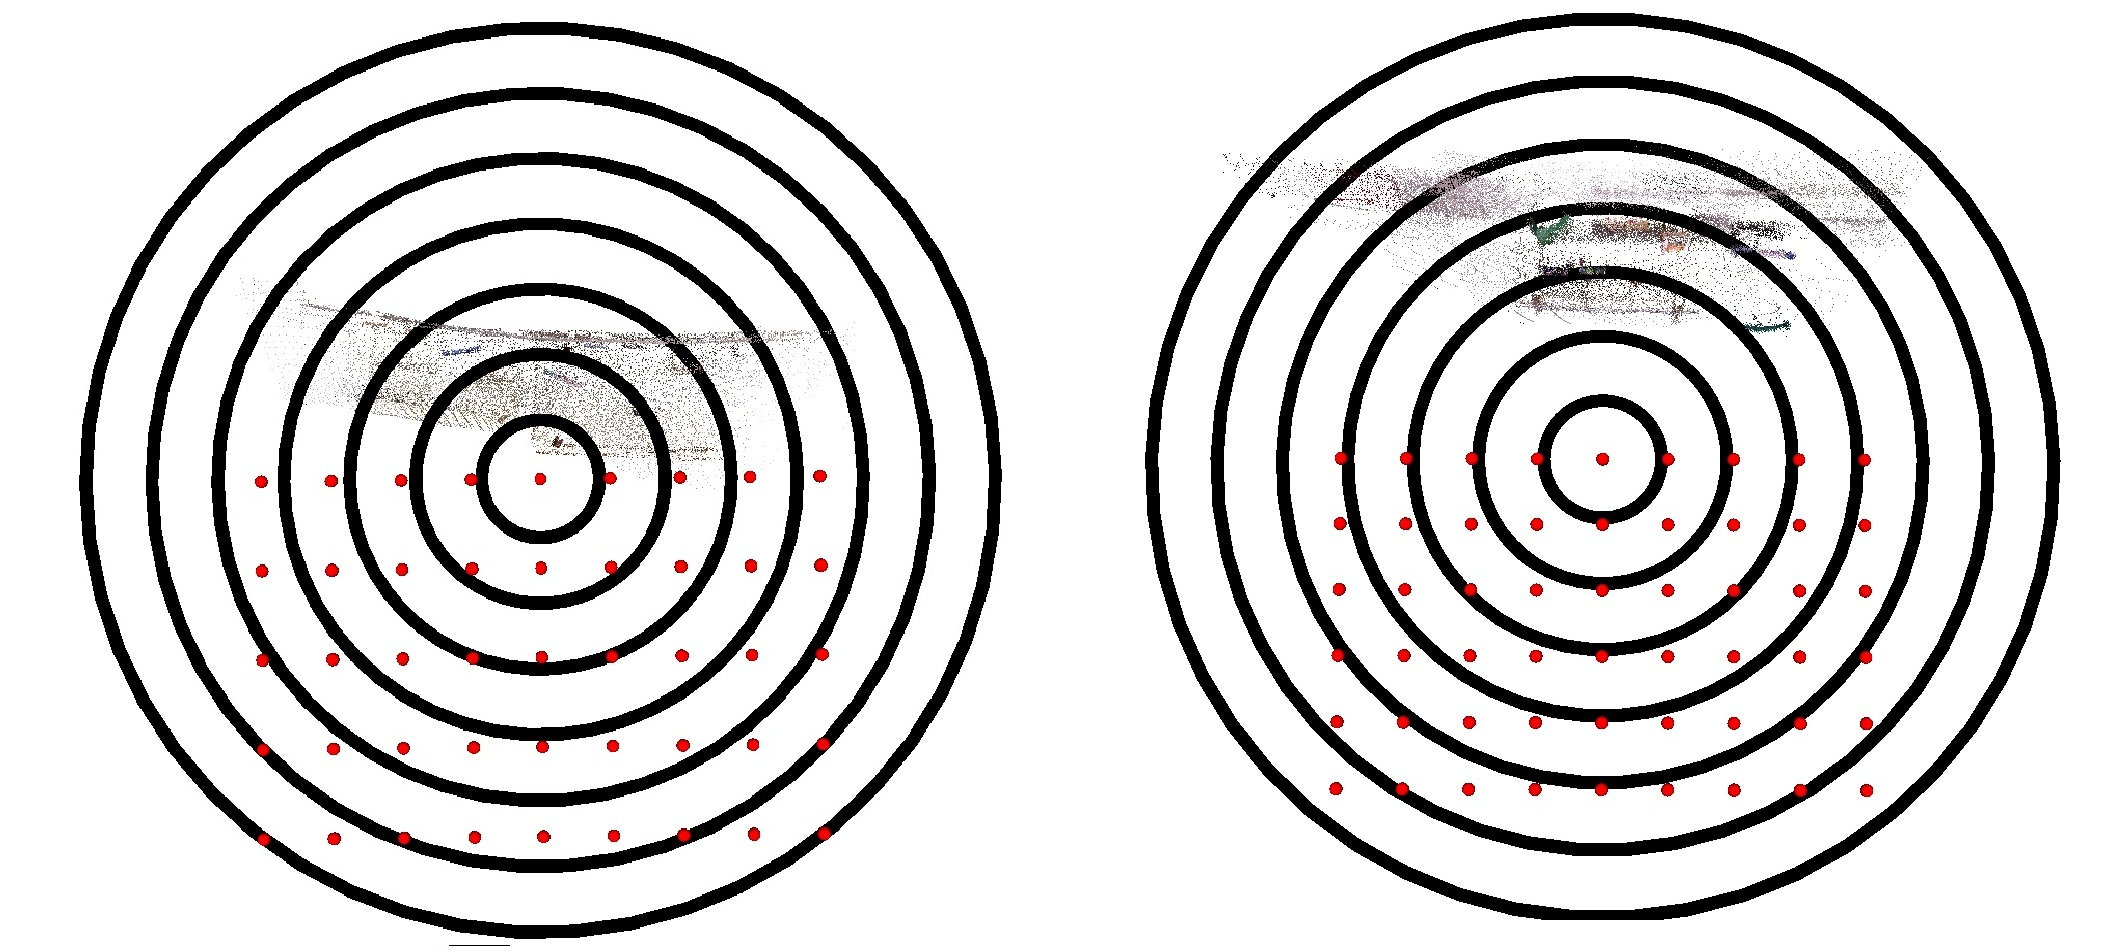
\includegraphics[width=1.0\textwidth]{figures/CoverDisk.jpg}
  \caption{依照同心圓的覆蓋算出每個半徑內的每張圖的特徵點平均數,左.控制環境 1 右.控制環境 2}
  \label{fig:CoverDisk}
\end{center}
\end{figure}

\begin{figure}
	\begin{center}
    \subfigure[控制環境 1.特徵點平均數量比較]{\label{fig:CoverDisk_Descriptor1}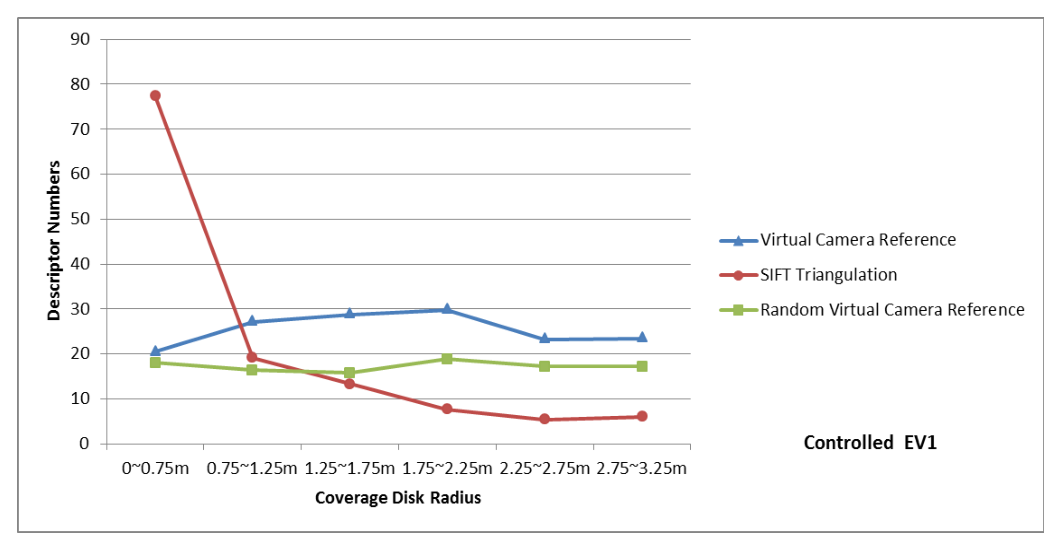
\includegraphics[width=0.9\columnwidth]{figures/Controlled_EV1_DescriptorNum.eps}}
    \subfigure[控制環境 2.特徵點平均數量比較]{\label{fig:CoverDisk_Descriptor2}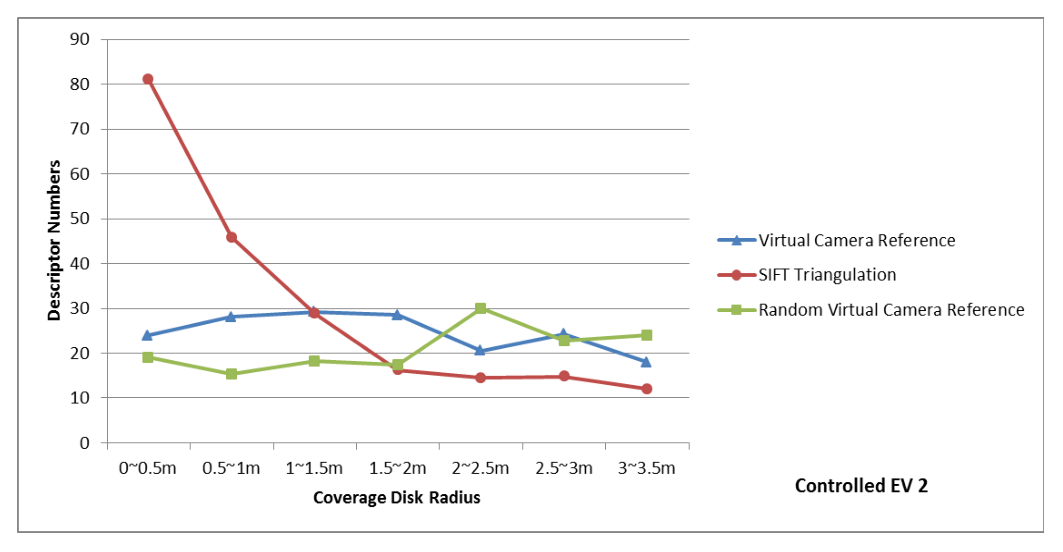
\includegraphics[width=0.9\columnwidth]{figures/Controlled_EV2_DescriptorNum.eps}}
	\end{center}
  \caption{特徵點數量趨勢圖,根據距離增加看出特徵點分布的數量差異情形}
  \label{fig:CoverDisk_DescriptorNum}	
\end{figure}

	這個實驗目的是要看出根據景物的距離增加與特徵點數量的關係圖,實驗的作法是先在待定位圖片的第一排中間設為圓心,如圖
\ref{fig:CoverDisk}所示。根據這個圓心將圓的半徑以間距距離的長度增加,像是控制環境1.中根據每個間距距離增加0.75m,控制環境2.中                                                                               
每個間距距離增加0.5m,依據每個圓之間所能覆蓋的特徵點位置做特徵點數量的總和並算出平均值,藉由圖中的趨勢看出特徵點數量的變化。下面根據
圖\ref{fig:CoverDisk_DescriptorNum}分析距離長度與特徵點數量作圖表分析。

	根據圖\ref{fig:CoverDisk_DescriptorNum}所示,
特徵點的數量變化,以虛擬影像格狀分布的數量為最穩定且平均數量較高的狀態,圖\ref{fig:CoverDisk_Descriptor1}在間距0.75 m的分布情形下,都有其對應的特徵點可供參考,
反觀SIFT影像特徵雖然在一開始可以找到多數的特徵點,但是隨著距離增加,數量逐步遞減,最後只有些許的特徵可以找出。圖\ref{fig:CoverDisk_Descriptor2}在間距0.5 m的分
布情形下,格狀分布的優勢較不明顯,SIFT平面影像特徵點數量趨勢下滑也趨於緩慢。

	圖\ref{fig:CoverDisk_Descriptor1}與圖\ref{fig:CoverDisk_Descriptor2}分析得出間距距離大,對格狀分布與隨機分布的影響差異越大,其中這些數量上的差異會影響之
後間距定位的成果。尤其在圖\ref{fig:CoverDisk_Descriptor1}間距0.75 m下的數量差異最為明顯,而格狀的虛擬相機分布其特徵點數量呈穩定的趨勢,比起隨機分布更能運在室內定
位上,改進資料蒐集不完全的問題。
	
\begin{figure}
	\begin{center}
    \subfigure[控制環境 1.間距定位平均誤差比較]{\label{fig:Distance_Error1}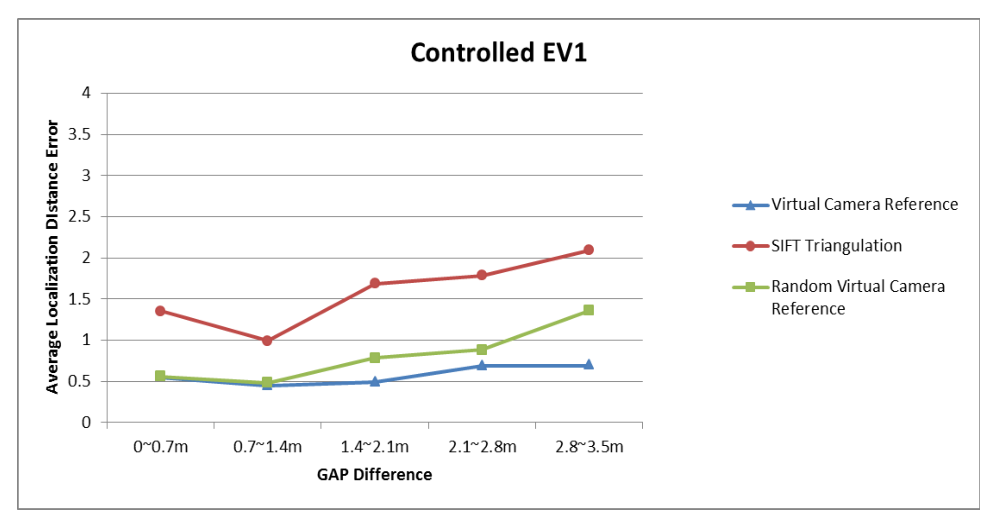
\includegraphics[width=0.9\columnwidth]{figures/Controlled_EV1_Localization_Distance_Error.eps}}
    \subfigure[控制環境 2.間距定位平均誤差比較]{\label{fig:Distance_Error2}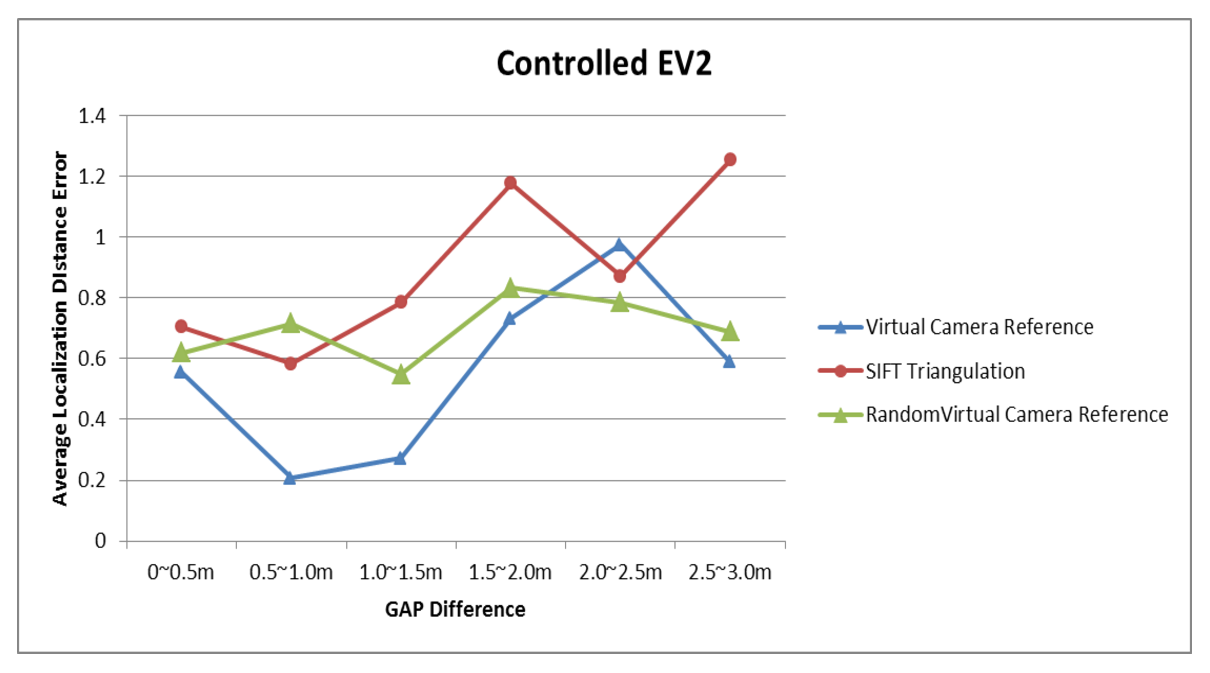
\includegraphics[width=0.9\columnwidth]{figures/Controlled_EV2_Localization_Distance_Error.eps}}
	\end{center}
  \caption{間距定位平均誤差趨勢圖,以每一橫排的待定位圖片平均誤差做計算,看出距離增加對定位誤差是否有影響}
  \label{fig:Localization_Distance_Error}	
\end{figure}	
	
\subsection{間距定位誤差趨勢}	
	
	以圖\ref{fig:Localization_Distance_Error}可看出,以每一橫排的待定位圖片的平均誤差分布,根據每一個不同的間距,虛擬相機圖片定
位比一般相機所做出的影像定位誤差都有改善,尤其以圖\ref{fig:Distance_Error1}格狀分布的3D虛擬影像改善最為明顯。根據我們的方法,我們想要模擬在不同的角度及位置產生3D虛
擬影像,比起一般的傳統影像有更多可以做特徵點匹配的相片可供使用。

傳統的平面影像定位所做出的資料庫中,對於景物比較遠的照片並沒有資訊提供,只
能利用拘限在景物較近的照片可供定位,但是少許的特徵點使得定位誤差更加放大,所以照圖中趨勢來看,距離一增加,定位誤差就會加大。但是在3D虛擬影
像不會因為距離的增加,導致定位誤差增加。除了3D虛擬影像可以增加更多可以被匹配的相片以外,好的虛擬相機分布,也可以產生更多的特徵點可以被匹配
。以隨機分布與格狀分布來說,隨機分布的3D虛擬相片雖然有改善,但沒有比格狀分布的虛擬相片改善來的明顯。

在我們的方法中,我們定位會參考照相機所
在的位置,所以定位的位置都會在相機位置的附近,隨機分布可能會造成某些區域的相機分布過於集中,某些相機卻又過於分散的情況發生。所以在隨機虛擬
相機分布的定位其實就跟平面相機分布的定位分布差不多,差別在於相片角度會避開障礙物,但不會均勻分布在環境中;格狀平均分布的攝影機位置,就會均
於分布在環境內,而對於影像特徵點匹配上比隨機分布來的更有幫助。


\subsection{定位精準度覆蓋率以及平均定位誤差分布情況}	
	
\begin{figure}
	\begin{center}
	\rotatebox{90}{
	\subfigure[控制環境 1.]{\label{fig:Controlled_EV1_Result}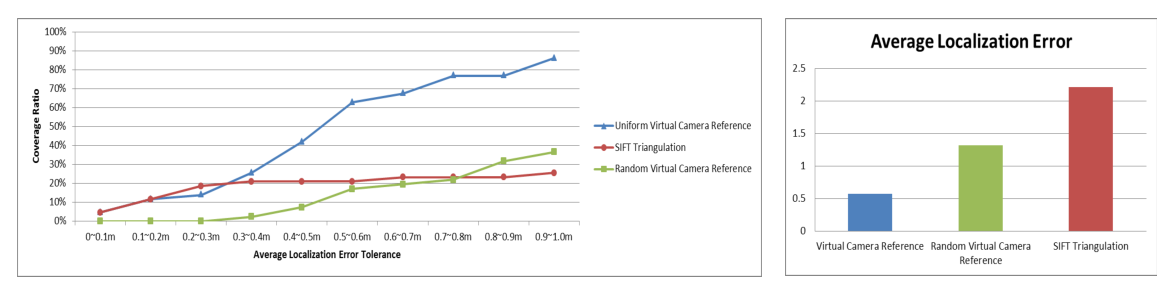
\includegraphics[width=1.2\columnwidth]{figures/Controlled_EV1_Result.eps}}
	}
	\rotatebox{90}{
	\subfigure[控制環境 2.]{\label{fig:Controlled_EV2_Result}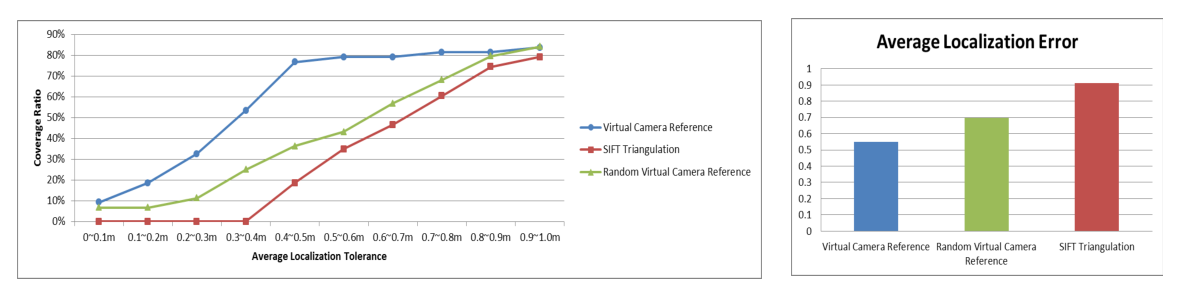
\includegraphics[width=1.2\columnwidth]{figures/Controlled_EV2_Result.eps}}
	}
	%\subfigure[平均定位誤差]{\label{fig:Controlled_AVG_Error}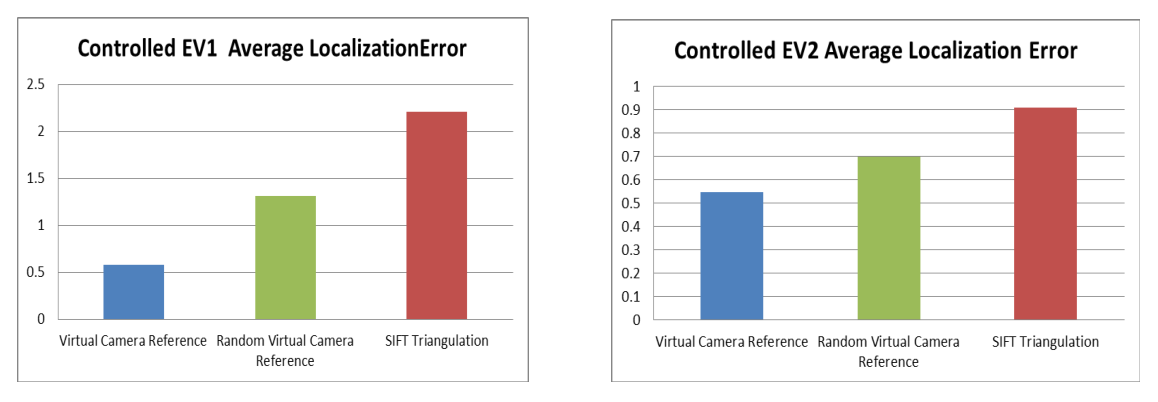
\includegraphics[width=1.0\columnwidth]{figures/Controlled_Average_Result.eps}}
	\end{center}
  \caption{控制環境下定位精準度覆蓋率以及平均定位誤差成果分析,(a),(b)圖為誤差容忍範圍下,可定位成功的覆蓋率分布情形}
  \label{fig:Controlled_EV_Result}	
\end{figure}	

\begin{figure}
\begin{center}
  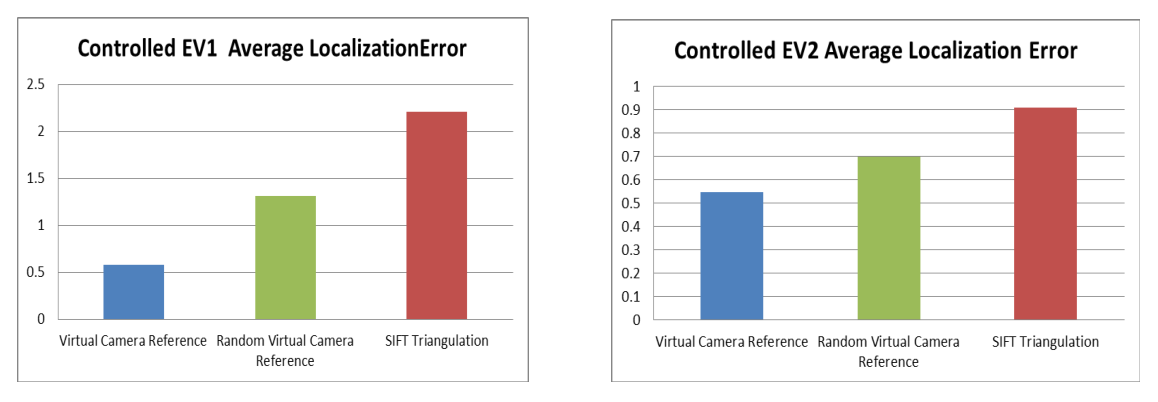
\includegraphics[width=1.0\textwidth]{figures/Controlled_Average_Result.eps}
  \caption{控制環境下定位平均誤差}
  \label{fig:Controlled_AVG_Error}
\end{center}
\end{figure}

	研究發現與景物的距離越遠在3D虛擬影像定位並不會影響誤差,整體來看,對定位的覆蓋率也有一定的提升。根據圖\ref{fig:Controlled_EV1_Result}與圖\ref{fig:Controlled_EV2_Result}
所示,在格狀分布
的3D虛擬相機定位在誤差0.5 m左右有超過$60\%$的覆蓋率,但隨機分布的虛擬相機以及2D平面影像定位坐落在$20\% \sim 30\%$左右上下,表示相機的分
布影響定位結果的好壞,這也是我們讓照相機格狀分布平均的原因。藉由均勻取得的定位資訊,改善影像蒐集中容易遺漏的邊緣及死角,確保在定位時,能保留定位
資料的完整性,避免相機分布不均導致資料遺漏的情形發生。

回到圖\ref{fig:CoverDisk_Descriptor1}來看,在1.75 m以後的隨機虛擬相
片所找出特徵點平均數量比起格狀分布虛擬相片所找出的特徵點數量少上許多,而在圖\ref{fig:Distance_Error1}來看,每個間距的定位平均誤差,
格狀分布都比隨機分布的誤差好上許多。所以當以誤差在0.6 m以內的覆蓋率來說,隨機分布的虛擬相片並沒有產生比較好的定位覆蓋率,但以格狀分布的
虛擬相片定位覆蓋率與2D影像定位覆蓋率相比,結果好上許多。

這說明虛擬相機分布的位置,影響了虛擬相片的品質,
平均定位誤差平均定位的誤差以格狀的虛擬影像為物誤差為最低,2D影像定位的誤差為最高,改善了整體定
位的平均誤差。最後以圖\ref{fig:Controlled_AVG_Error}來看,格狀分布的虛擬影像定位平均誤差皆
為最小,在單一景物的定位環境實驗下,研究方法能夠對定位平均誤差與覆蓋率作改善,也證實景物不會因相機
距離增加導致誤差發生。最後在一般室內環境下根據定位誤差與覆蓋率作實驗分析。

%2. Indoor Localization
\section{一般室內環境定位實驗}

	在控制環境下,改善了定位的覆蓋率與精準度,在這章節將在一般室內環境下進行定位測試。我們將室內定位環境分成兩種情境:(1)
居家客廳 ,(2) 居家廚房與 ,分別在這兩種環境下進行定位實驗。在一般室內定位主要進行定位覆蓋率與定位平均誤差測試。
	
	在室內定位的情況下,拍攝待定位照片的方法依據環境情況而定。待定位照片拍攝方法是依照人能夠活動的範圍作依據,在這些區域進行
格點分布拍攝,如圖\ref{fig:Indoor_EV1_query}與圖\ref{fig:Indoor_EV2_query}所示。每張待定位圖片的間距距離為0.5公尺,
照片數量根據環境大小而定,平均在30張上下。虛擬照片依據間距距離,取出不同數量的虛擬相機。因為考量不同環境的景物分布,每組相機位置
分別拍攝兩種不同的角度,最後根據虛擬相機拍攝出的照片作影像定位。除了與2D影像定位方法做比較之外,分別測試在不同虛擬照片資料數量的
定位情形。
		
\begin{table}[htbp]
  \centering
  \caption{室內定位環境大小分布}
    \begin{tabular}{rrr}
    \toprule
    實驗設定 :  & 客廳 & 廚房 \\
    \midrule
    待定位照片數量 : & 35 張  & 30 張 \\
    間距距離 : & 0.5m & 0.5m \\
    環境長度 : & 3.8m & 4.1m \\
    環境寬度 : & 4.1m & 3.2m \\
    \bottomrule
    \end{tabular}%
  \label{table:Indoor EV parameters}%
\end{table}%
	
	
	表2.2 記錄了不同室內定位環境的設定,分別在不同環境下進行實驗,每個環境的虛擬相機位置均採用格狀分布。圖\ref{fig:Indoor_EV_and_Query}
記錄當時點雲環境的建置以及待定位照片的位置分布。點雲的建置是利用Kinect環繞室內環境四周所拍攝,再利用這些拍攝的圖片,當作平面2D影像定位
所需的影像資料庫。接下來分別以不同虛擬相機照片的數量與平面2D影像做實驗比較分析。
	
\subsection{定位覆蓋率與定位平均誤差分析比較}

\begin{figure}
	\begin{center}
	\subfigure[定位環境 1.客廳環境]{\label{fig:Indoor_EV1}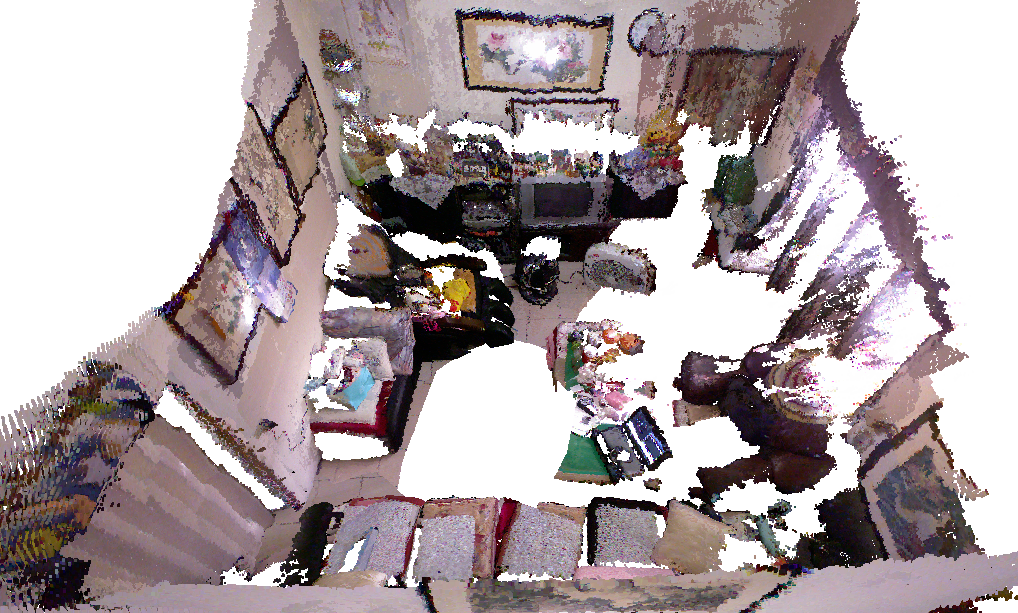
\includegraphics[width=0.45\columnwidth]{figures/snapshot00.jpg}}
	\subfigure[定位環境 2.廚房環境]{\label{fig:Indoor_EV1}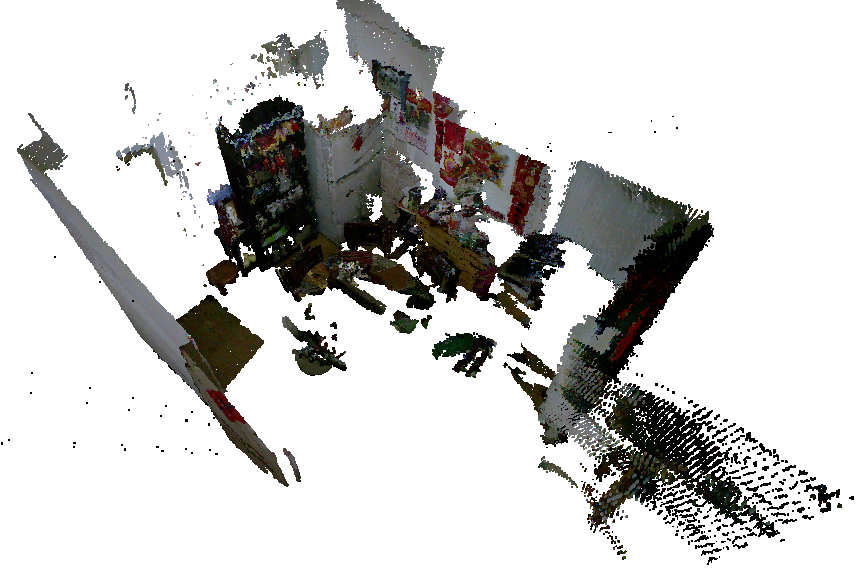
\includegraphics[width=0.45\columnwidth]{figures/snapshot01.jpg}}
    \subfigure[定位環境 1.客廳 待定位照片分布位置]{\label{fig:Indoor_EV1_query}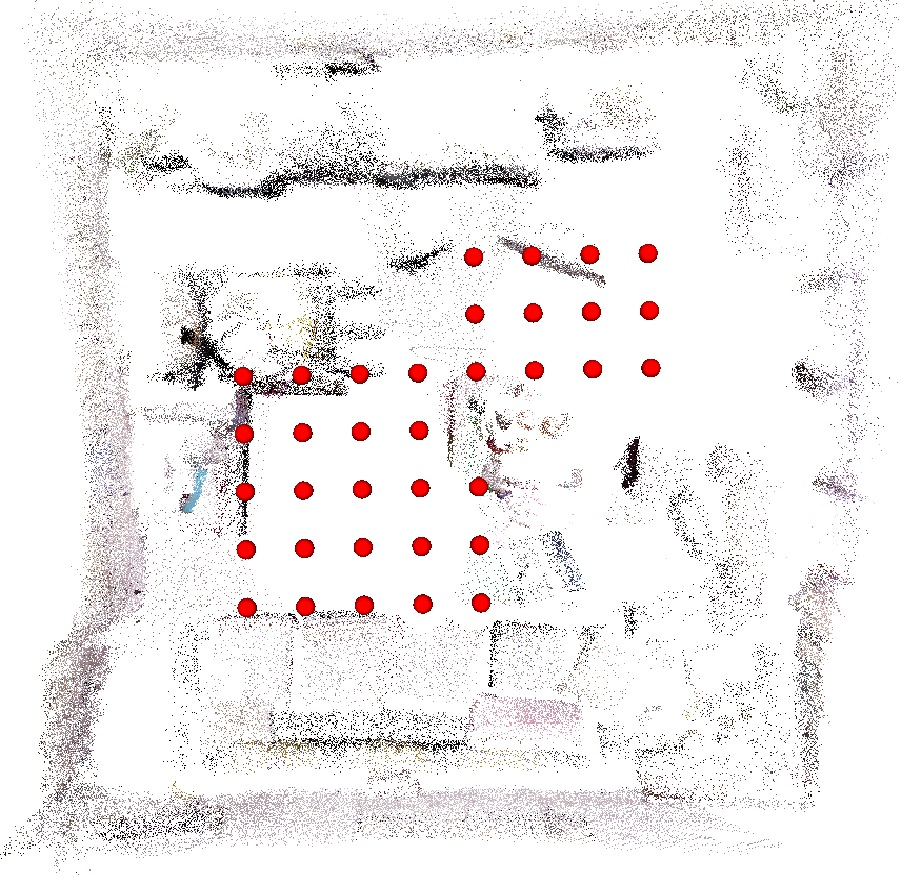
\includegraphics[width=0.4\columnwidth]{figures/LivingRoom_QueryPose.jpg}}
    \subfigure[定位環境 2.廚房 待定位照片分布位置]{\label{fig:Indoor_EV2_query}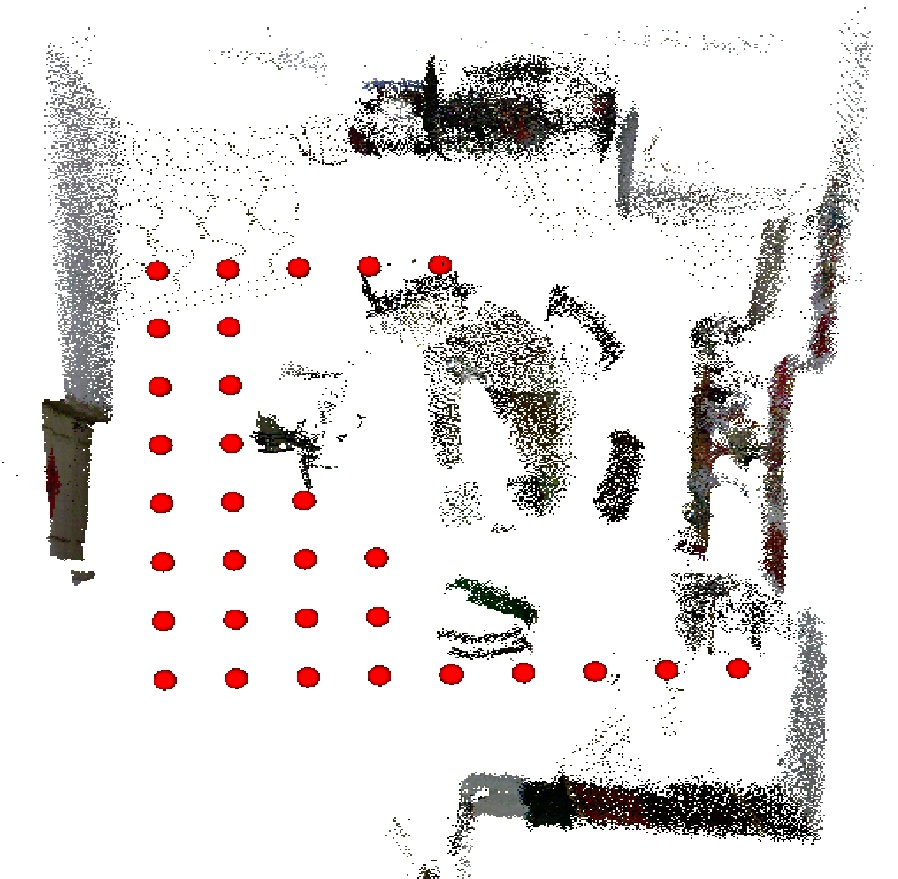
\includegraphics[width=0.4\columnwidth]{figures/Kitchen_QueryPose.jpg}}
	\end{center}
  \caption{室內定位環境與待定位照片分布位置}
  \label{fig:Indoor_EV_and_Query}	
\end{figure}		

\begin{figure}
	\begin{center}
	{\rotatebox{90}{
		\subfigure[客廳環境]{\label{fig:LivingRoom_Result}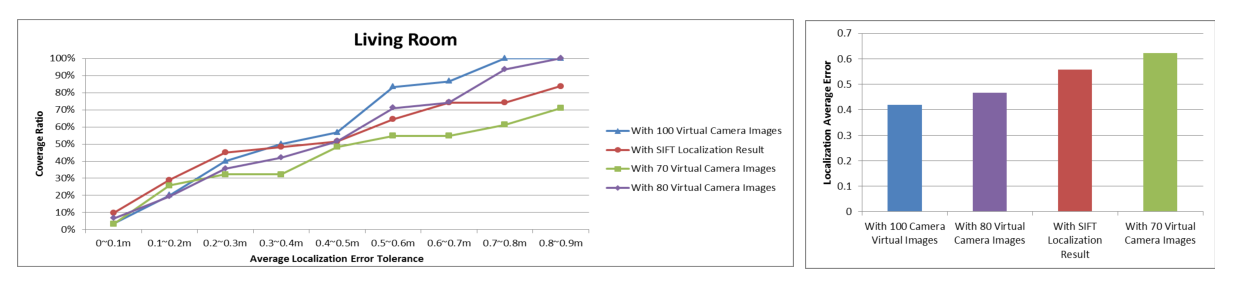
\includegraphics[width=1.2\columnwidth]{figures/Indoor_LivingRoom_Result.eps}}
		}
		\rotatebox{90}{
		\subfigure[廚房環境]{\label{fig:Kitchen_Result}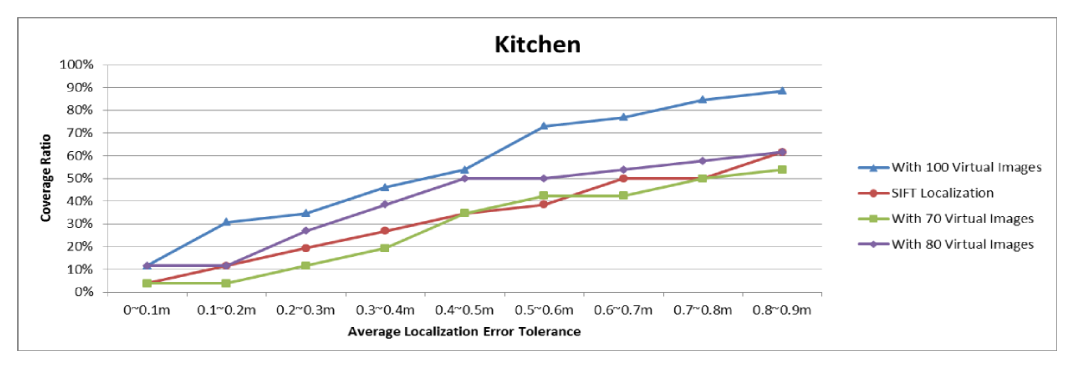
\includegraphics[width=1.2\columnwidth]{figures/Indoor_Kitchen_Result.eps}}
		}
		%\subfigure[平均定位誤差]{\label{fig:Indoor_EV2}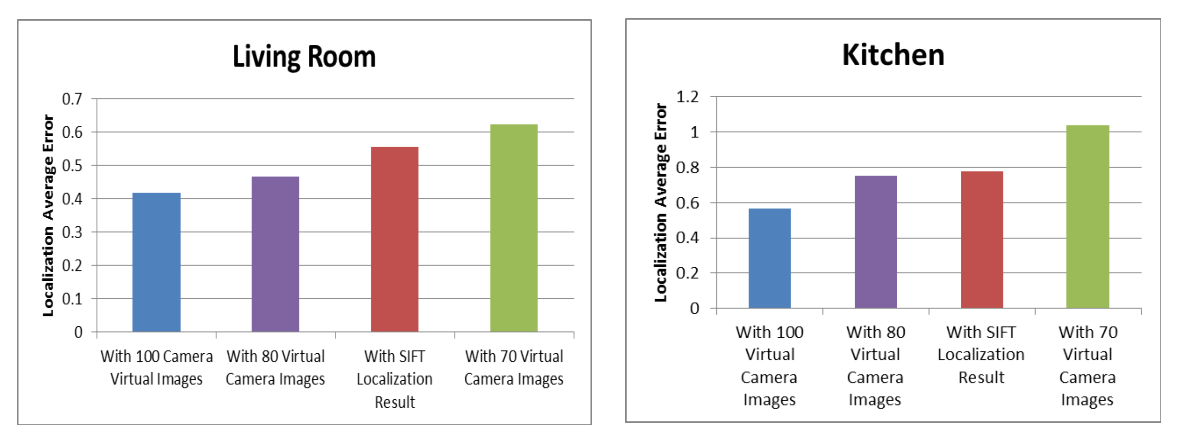
\includegraphics[width=1.0\columnwidth]{figures/Indoor_Average_Result.eps}}
		}
	\end{center}
  \caption{室內環境定位成果,上圖為誤差容忍範圍下定位成功覆蓋率,在容忍範圍下覆蓋率分布的變化,(a)為客廳環境,(b)為廚房環境}
  \label{fig:Indoor_EV_and_Query}	
\end{figure}	

\begin{figure}
\begin{center}
  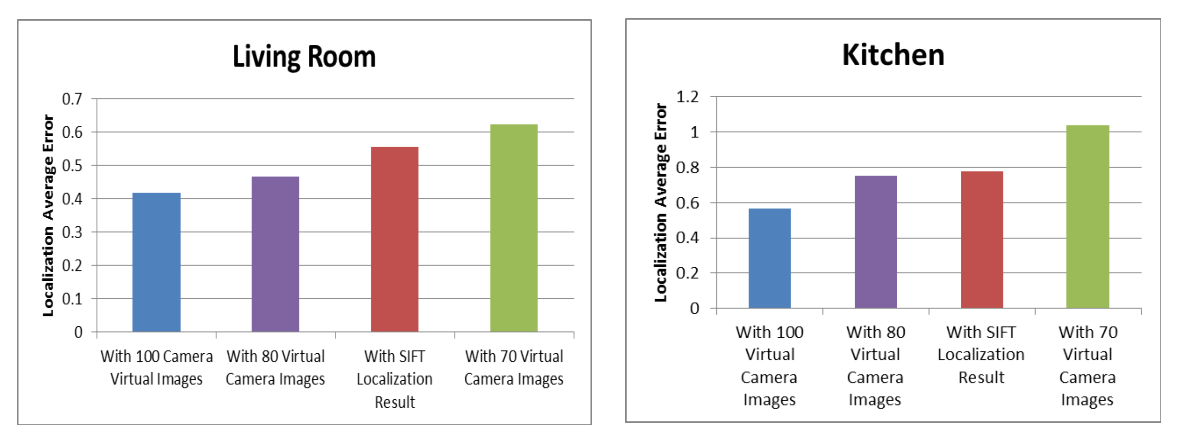
\includegraphics[width=1.0\textwidth]{figures/Indoor_Average_Result.eps}
  \caption{控制環境下定位平均誤差}
  \label{fig:Indoor_AVG_Error}
\end{center}
\end{figure}

		在室內定位的環境下,特徵點分布的數量,以及環境內觀測物的不同對定位結果增加許多變動因素。為了使定位結果能夠量化比較,我們將實驗結果分成(1).定位精準度
	覆蓋率,與(2).平均定位誤差兩個指標來分析成果。在圖\ref{fig:Indoor_EV_and_Query}之中來看,橫坐標表示定位誤差的容忍範圍,縱座標代表在這個誤差
	範圍下的定位成功率,以三種不同虛擬照片的數量與傳統2D影像照片做實驗比較。
	
		以覆蓋率來看,100張虛擬照片的定位結果為最好,代表取得越多點雲環境的資料,定位的改善越明顯。因為在每個相機位置上,我們取出兩張虛擬照片,所以在環境中總共有
	50個虛擬相機位置作比較,分別與40個與35個相機位置相比,有更多定位參考的依據。則平面2D影像因為只有一部分的環境參考依據,所以在定位覆蓋率與平均誤差,都比100張與
	80張虛擬照片定位成果來的差。以\ref{fig:LivingRoom_Result}來看,誤差範圍在$0.5m \sim 0.6m$之間的覆蓋率,以100張虛擬照片覆蓋率最高,有$80\%$左右的定位成功率,但是平面
	2D影像只有$60\%$左右的成功率,增加了$20\%$的覆蓋率。
	
		以平均誤差來說也有改善,在上個章節中我們發現平面2D影像定位誤差會有不穩定的情況發生,這種情況增加了整
	體的平均定位誤差,而在虛擬影像定位因為誤差會穩定在$1m$以內的範圍內,所以也會降低平均定位誤差。在圖\ref{fig:Indoor_AVG_Error}來看,室內環境下的平均定位誤差也獲得改善,而大多
	的平均誤差都可控制到0.5 m以下,以虛擬影像的平均定位誤差來說,與平面影像定位相比,當大於40組虛擬相機位置時,都可以改善平均定位誤差。
	
		從兩個定位環境下以圖\ref{fig:Indoor_EV1_query}與圖\ref{fig:Indoor_EV2_query}分別看兩個待定位圖片分布的情形,得知在廚房的環境的待定位圖片分布偏向於同一側,
	另一側因為障礙物阻擋,對於實際相機取得較為困難。因為平面影像定位的環境資料缺乏,導致定位誤差上升,尤其以兩個定位環境互相比對最為明顯。但整體來說,100張虛擬影像所取得定位
	成果都最為穩定,說明虛擬影像可以在一定的數量下可以補足環境資訊的缺乏,藉由優化相機角度增加影像的相關性,在相機無法拍攝的位置取得影像及避開障礙物,使得整體覆蓋率與誤差都能
	改善。



%\chapter{Conclusions and Future Work}
%\label{sum}
%%\section{Conclusion and Future Work}\label{sum}

We proposed a 3D face reconstruction approach with a
color image in this paper. Compared with methods considering
grayscale images, the proposed approach uses multiple image
factors including the color information in establishing tensor
models with respect to images and corresponding depths.
A CCA-based mapping between image and depth tensors
is built, which bonds crucial information that benefits the
reconstruction. Once the mapping is constructed, 3D faces can
be reconstructed from a single color image with the help of
tensor models. The proposed approach also works when the
input face image is captured under different lighting conditions and poses. Experiment results show that the proposed method produces better outcome due to the inclusion of color channels in the multi-factor consideration. 


% back pages 後頁
% 包括參考文獻、附錄、自傳 
% 實際內容由backpages資料夾下
%    my_bib.bib, my_appendix.tex, my_vita.tex
% 決定
% ntust_backpages.tex 此檔只提供整體架構的定義,不需更動
% 在撰寫各章草稿時,可以把此部份「關掉」,以節省無謂的編譯時間。
%
% this file is encoded in utf-8
% v2.0 (Apr. 5, 2009)

%%% 參考文獻
\newpage
\phantomsection % for hyperref to register this
\addcontentsline{toc}{chapter}{\nameRef}
\renewcommand{\bibname}{\protect\makebox[5cm][s]{\nameRef}}
%  \makebox{} is fragile; need protect
\bibliographystyle{IEEEtran}  % 使用 IEEE Trans 期刊格式
\bibliography{ref}


%%% 附錄
%%
% this file is encoded in utf-8
% v2.0 (Apr. 5, 2009)
%%% 每一個附錄 (附錄甲、附錄乙、...) 都要複製此段附錄編排碼做為起頭
%%% 附錄編排碼 begin >>>
\newpage
\chapter*{附錄甲:MATLAB / Octave 程式列表} % 修改附錄編號與你的附錄名
\phantomsection % for hyperref to register this
\addcontentsline{toc}{chapter}{附錄甲:MATLAB / Octave 程式列表} %建議此內容應與上行相同
%\setcounter{chapter}{0}  %如果用的是 TeXLive2007 則打開此行以避免錯誤
\setcounter{equation}{0} 
\setcounter{figure}{0} 
\setcounter{footnote}{0} 
\setcounter{section}{0} 
\setcounter{subsection}{0}
\setcounter{subsubsection}{0}
\setcounter{table}{0} 
\renewcommand{\thechapter}{甲} % 如果是附錄乙,則內容應為{乙}
%%% <<< 附錄編排碼 end

% 附錄內容開始
% 納入程式源碼
\lstinputlisting{example_prog_list.m}


\begin{equation}\sum_{k=1}^{n} k = \frac{n(n+1)}{2}\end{equation}

%%% 如果有附錄乙、丙、...,則在此繼續加上「附錄編排」碼
% 每一個附錄會自動以新頁開始

%%% 自傳
%\newpage
%\chapter*{\protect\makebox[5cm][s]{\nameVita}} % \makebox{} is fragile; need protect
%\phantomsection % for hyperref to register this
%\addcontentsline{toc}{chapter}{\nameVita}
%本人生於 1981 年 1 月 1 日,在桃園內壢。家裡經營電器行,上有一位姊姊。從小就喜歡拆解店裡收回的報廢家電用品,練就了一身好手藝與探究一切的好奇心。

國小就讀平鎮國小。由於把供應全校用水的抽水馬達拆開研究裝不回去,造成全校停水,廁所污穢不堪。被校長處罰掃廁所一個星期。那真是我少時年幼無知的一頁插曲。



\end{document} 
